\clearpage
\section{HEEP ID efficiency and scale factor}\label{sec:Zprime_SF}
The MC samples used for High Energy Electron Pair (HEEP) selection efficiency and scale factor measurement are listed in Table \ref{tab:HEEPSF-samples}
\begin{table}[htp]
  \begin{center}
\small
\smallskip\noindent
\resizebox{\linewidth}{!}{%
\begin{tabular}{|l|l|l|}
\hline
sample                                                                  & xsection(pb) & comments \\
\hline
\hline
DYToEE\_NNPDF30\_ 13TeV-powheg-pythia8                                 & 1921.8   & for 2016 $Z\rightarrow ee$     \\
\hline
DYJetsToLL\_M-50\_TuneCUETP8M1\_13TeV-madgraphMLM-pythia8              & 5765.4   & for 2016 $Z\rightarrow\tau\tau$        \\
DYJetsToLL\_M-50\_TuneCP5\_13TeV-amcatnloFXFX-pythia8                  & 5765.4   & for 2017 $Z\rightarrow ee$, $Z\rightarrow\tau\tau$        \\
\hline
WJetsToLNu\_TuneCUETP8M1\_13TeV-madgraphMLM-pythia8                    & 61526.7  & for 2016, 2017       \\
\hline
TT\_TuneCUETP8M2T4\_13TeV-powheg                                        & 831.76  & for 2016             \\
TTTo2L2Nu\_TuneCP5\_13TeV-powheg-pythia8                                & 87.31   & for 2017             \\
TTToSemiLeptonic\_TuneCP5\_PSweights\_13TeV-powheg-pythia8              & 366.6   & for 2017             \\
ST\_tW\_top\_5f\_inclusiveDecays\_13TeV-powheg-pythia8                  & 35.6    & for 2016, 2017       \\
ST\_tW\_antitop\_5f\_inclusiveDecays\_13TeV-powheg-pythia8              & 35.6    & for 2016, 2017        \\
\hline
GJets\_HT-40To100\_TuneCUETP8M1\_13TeV-madgraphMLM-pythia8              & 20790   & for 2016, 2017         \\
GJets\_HT-100To200\_TuneCUETP8M1\_13TeV-madgraphMLM-pythia8             & 9238    & for 2016, 2017         \\
GJets\_HT-200To400\_TuneCUETP8M1\_13TeV-madgraphMLM-pythia8             & 2305    & for 2016, 2017         \\
GJets\_HT-400To600\_TuneCUETP8M1\_13TeV-madgraphMLM-pythia8             & 274.4   & for 2016, 2017        \\
GJets\_HT-600ToInf\_TuneCUETP8M1\_13TeV-madgraphMLM-pythia8             & 93.46   & for 2016, 2017         \\
\hline
WW\_TuneCUETP8M1\_13TeV-pythia8                                         & 118.7   & for 2016, 2017         \\
WZ\_TuneCUETP8M1\_13TeV-pythia8                                         & 47.13   & for 2016, 2017         \\
ZZ\_TuneCUETP8M1\_13TeV-pythia8                                         & 16.523  & for 2016, 2017         \\
\hline
\end{tabular}}
\caption{MC samples used in HEEP efficiency and scale factor study}
\label{tab:HEEPSF-samples}
  \end{center}
\end{table}


\subsection{Tag and probe method}
\label{subsubsec:Same_sign_method}
To calculate the efficiency of a certain selection we use a method called 'tag and probe' using Z $\rightarrow$ ee events. This method starts by searching for a good electron, 'tag', which satisfies certain types of criteria. Then the efficiency of interest is measured testing the cuts on a second electron candidate called 'probe' electron. For this study, we measure HEEP ID efficiency and scale factor.

Tag is required to fulfill the following conditions and is paired with every other gsf electron candidate in the event that passes the $E_{T}$ and $\eta$ acceptance cuts of the HEEP ID (probe).
\begin{itemize}
  \item[$\bullet$] tag must pass the HEEP ID
  \item[$\bullet$] tag must be a barrel electron
  \item[$\bullet$] tag must be matched to the \texttt{HLT\_Ele27\_eta2p1\_WPTight} (\texttt{HLT\_Ele35\_WPTight}) trigger in data in 2016 (2017)
\end{itemize}
The invariant mass of the tag and probe must satisfy $70 < m(ee) < 110 ~\mathrm{GeV/c^{2}}$. If there are multiple tag and probe candidates in an event then all pairs are selected.
When there are two tags in a pair, both are considered to also be probes.
What we get is a very clear peak around the mass of the Z boson.
Therefore, we are confident that the electrons we have chosen are in fact products of a Z boson decay and are real electrons although there are low contamination from other standard model backgrounds.

The efficiency is defined as
\begin{equation}
\label{SF:eq:eff}
\epsilon_{\text{HEEP}} = \frac{N_{\text{passing probes}}}{N_{\text{all probes}}}
\end{equation}
where $N_{\text{all probes}}$ is the total number of all selected probes and $N_{\text{passing probes}}$ is the total number of selected probes which pass HEEP ID selection criteria. The efficiency can be measured in data and MC as a function of different variables like electron $E_{T}$, $\eta$, $\phi$, etc.

For finding HEEP ID efficiency in data, events are selected from SingleElectron dataset using \texttt{HLT\_Ele27\_eta2p1\_WPTight} (\texttt{HLT\_Ele35\_WPTight}) trigger in 2016 (2017).

For finding HEEP ID efficiency in MC, various MC samples are used which can be found in tables \ref{tab:HEEPSF-samples}. MC events are weighted using the trigger turn on curve of \texttt{HLT\_Ele27\_eta2p1\_WPTight} (\texttt{HLT\_Ele35\_WPTight}) path (see figure~\ref{fig:Ele27_2016} and ~\ref{fig:Ele35_2017} of section~\ref{sec:Other_HLT_efficiency}) to emulate the trigger efficiency instead of matching tag with the \\
\texttt{HLT\_Ele27\_eta2p1\_WPTight} (\texttt{HLT\_Ele35\_WPTight}) trigger object.
MC events are weighted to correct for differnce between data and MC pileup distribution according to the standard procedure.

The contribution of  QCD background, where tag and  probe are misidentified jets, is extracted from data using the 'same-sign' method.
In same-sign method, we use the fact that the probability of assigning positive or negative charge to the misidentified jet should be equal (LHC is proton proton collider and positive charged jets should be produced a bit more but we are not sensitive to that amount in this study).
Therefore, opposite sign and same sign tag and probe pairs are similar for QCD in total number and distribution shape for many variables. On the other hand, all other standard model processes have opposite sign electron pairs and do not contribute to same sign control region.

In Figure \ref{fig:SS_nominal_mee_2016}, the invariant mass distributions of selected tag and probe pairs are shown for all tag and probe pairs (top), tag and probe pairs in which probe passes HEEP ID selection cuts 'pass-pass' (middle) and tag and probe pairs in which probe fails passing  HEEP ID selection cuts 'pass-fail' (bottom). Due to the different ID efficiencies in barrel and endcaps, the invariant mass distribution of selected tag and probe pairs are separated for probe electrons in barrel and endcaps.
From Figure \ref{fig:SS_nominal_Et_2016} to \ref{fig:SS_nominal_PV_2016} (\ref{fig:SS_nominal_mee_2017} to \ref{fig:SS_nominal_PV_2017}) are invariant mass distributions of selected tag and probe pairs, $E_{T}$, $\eta$, $\phi$ of probes and number of primary vertex for the selected tag and probe pairs event in 2016 (2017).
\begin{figure}[htp]
  \begin{center}
    \begin{tabular}{cc}
      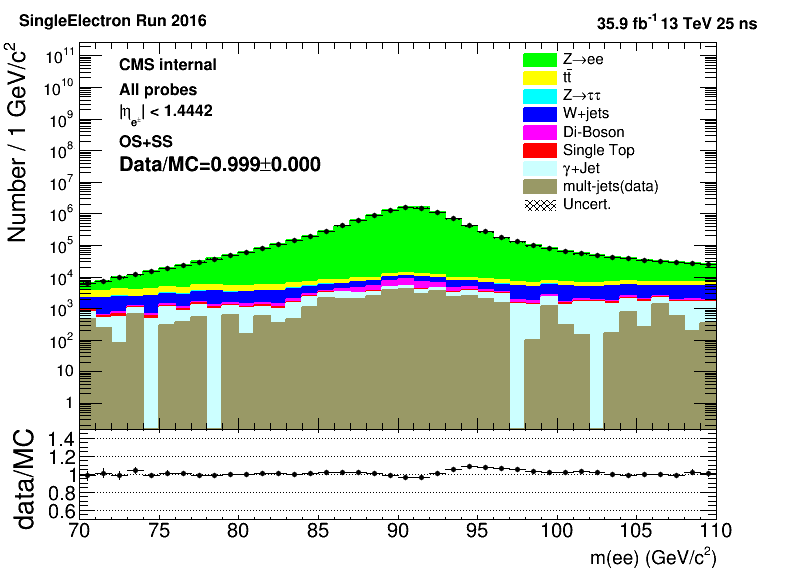
\includegraphics[width=0.45\textwidth]{figures/Zprime/2016/ScaleFactor/SameSign/nominal/stack_mee_Barrel_probes_PUW.png} &
      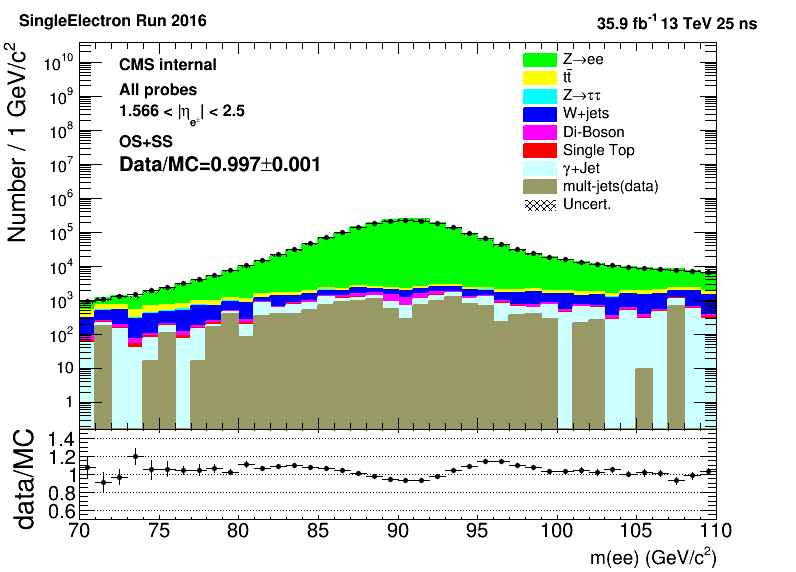
\includegraphics[width=0.45\textwidth]{figures/Zprime/2016/ScaleFactor/SameSign/nominal/stack_mee_Endcap_probes_PUW.png} \\
      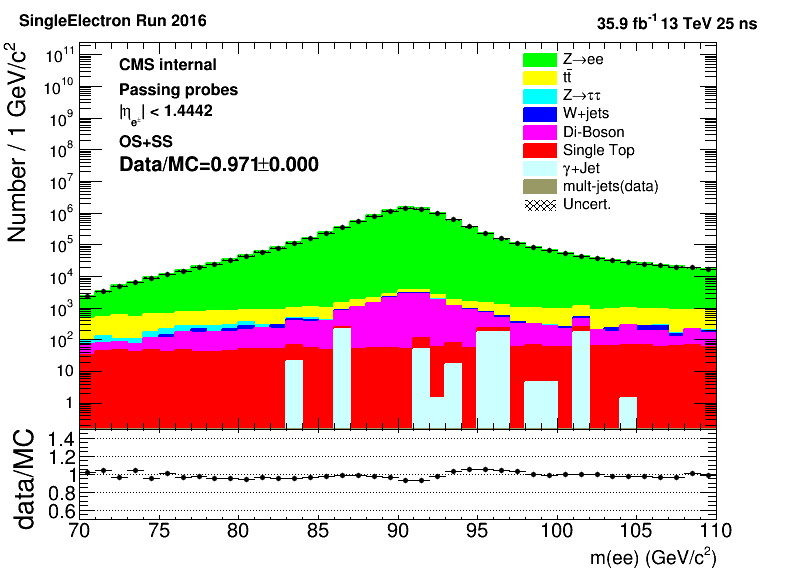
\includegraphics[width=0.45\textwidth]{figures/Zprime/2016/ScaleFactor/SameSign/nominal/stack_mee_Barrel_pass_PUW.png} &
      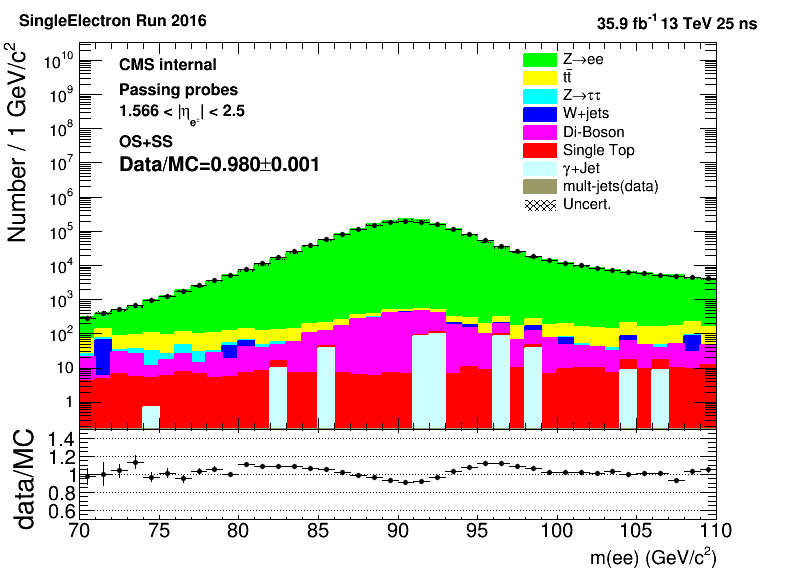
\includegraphics[width=0.45\textwidth]{figures/Zprime/2016/ScaleFactor/SameSign/nominal/stack_mee_Endcap_pass_PUW.png}\\
      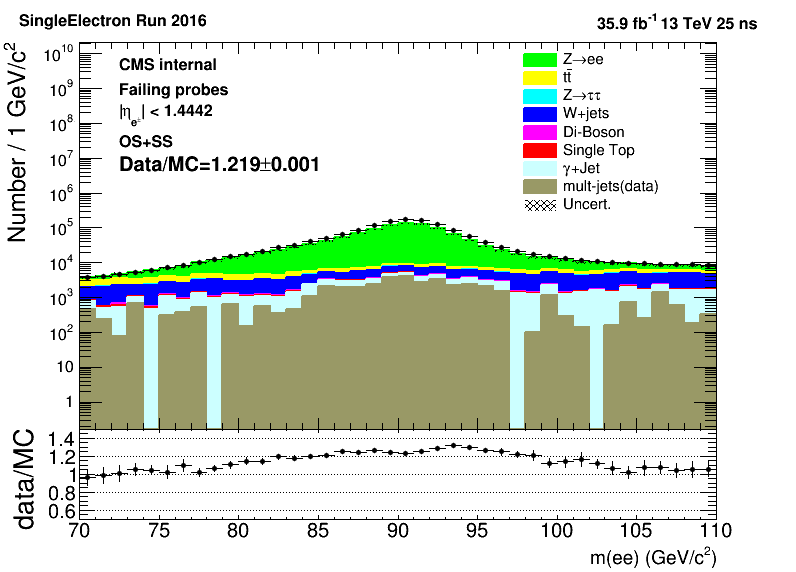
\includegraphics[width=0.45\textwidth]{figures/Zprime/2016/ScaleFactor/SameSign/nominal/stack_mee_Barrel_fail_PUW.png} &
      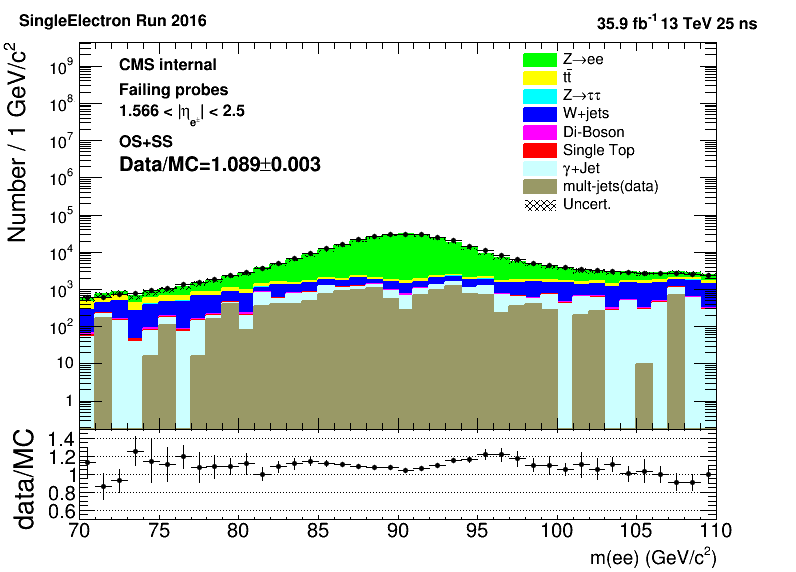
\includegraphics[width=0.45\textwidth]{figures/Zprime/2016/ScaleFactor/SameSign/nominal/stack_mee_Endcap_fail_PUW.png}
    \end{tabular}
    \caption{Invariant mass of tag and probe for probe in the barrel (left) and endcap (right) where all the probes are included (top), only passing probes are included (middle) and only failed probes are included (bottom) for 2016.}
    \label{fig:SS_nominal_mee_2016}
  \end{center}
\end{figure}
\begin{figure}[htp]
  \begin{center}
    \begin{tabular}{cc}
      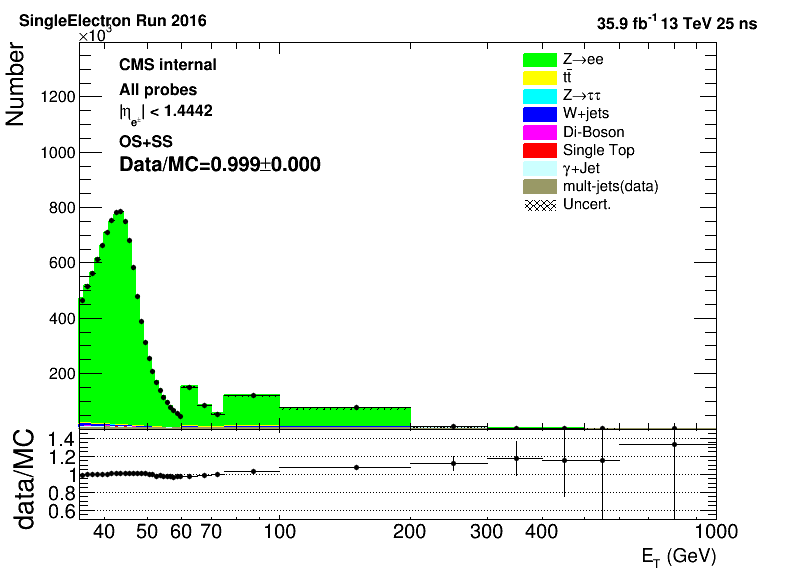
\includegraphics[width=0.45\textwidth]{figures/Zprime/2016/ScaleFactor/SameSign/nominal/stack_Et_Barrel_probes_PUW.png} &
      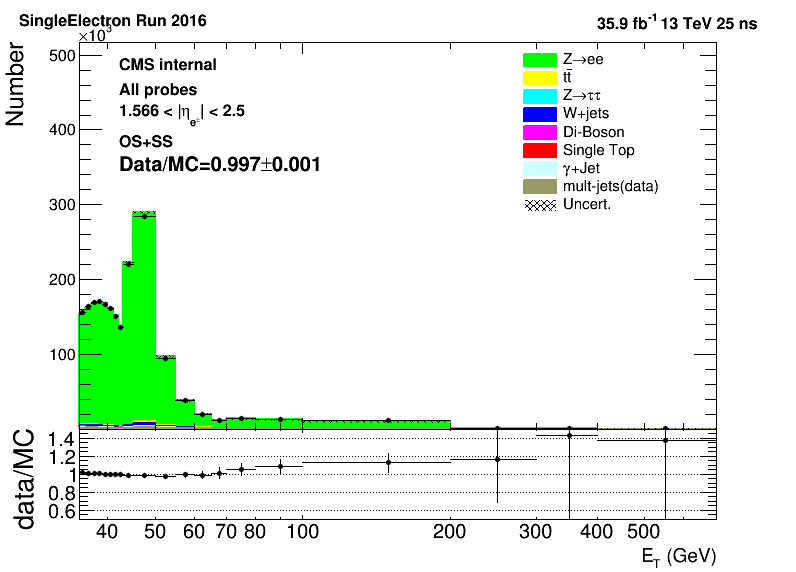
\includegraphics[width=0.45\textwidth]{figures/Zprime/2016/ScaleFactor/SameSign/nominal/stack_Et_Endcap_probes_PUW.png} \\
      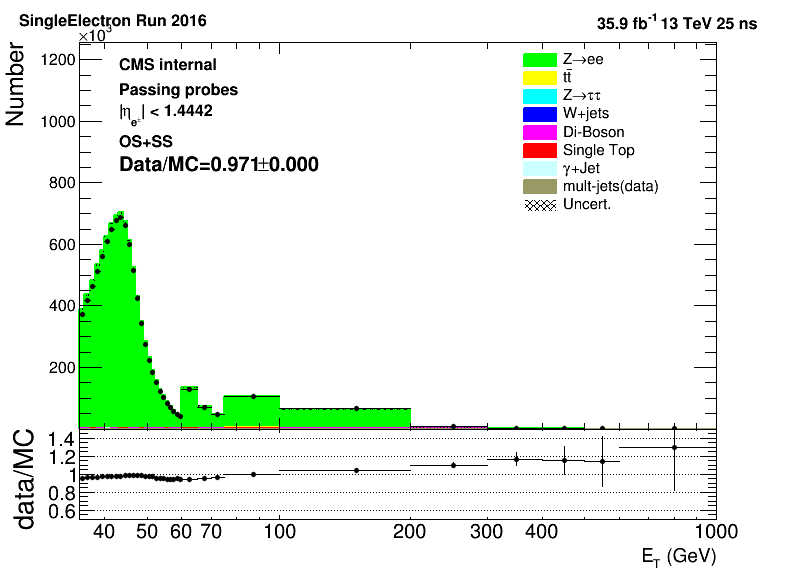
\includegraphics[width=0.45\textwidth]{figures/Zprime/2016/ScaleFactor/SameSign/nominal/stack_Et_Barrel_pass_PUW.png} &
      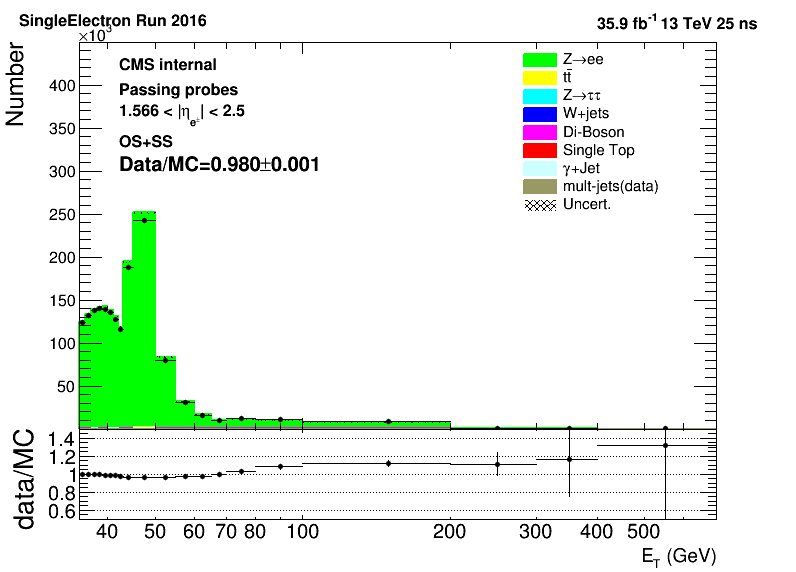
\includegraphics[width=0.45\textwidth]{figures/Zprime/2016/ScaleFactor/SameSign/nominal/stack_Et_Endcap_pass_PUW.png}\\
      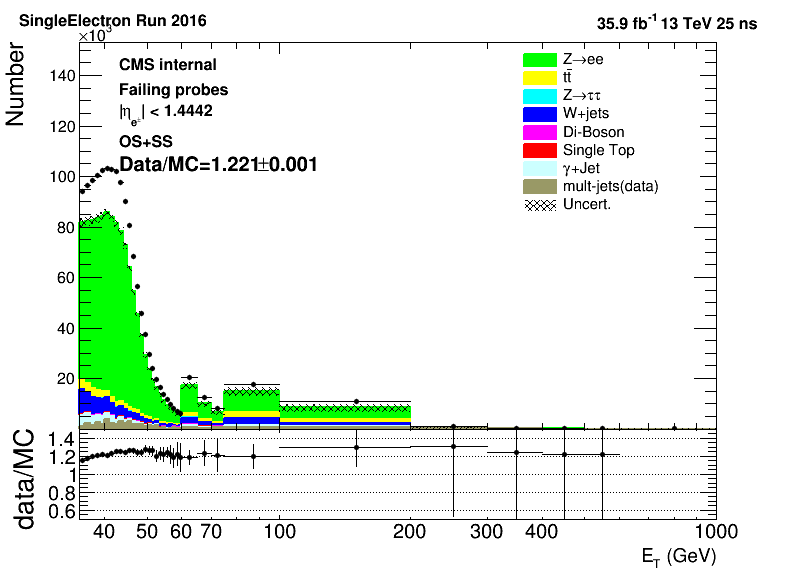
\includegraphics[width=0.45\textwidth]{figures/Zprime/2016/ScaleFactor/SameSign/nominal/stack_Et_Barrel_fail_PUW.png} &
      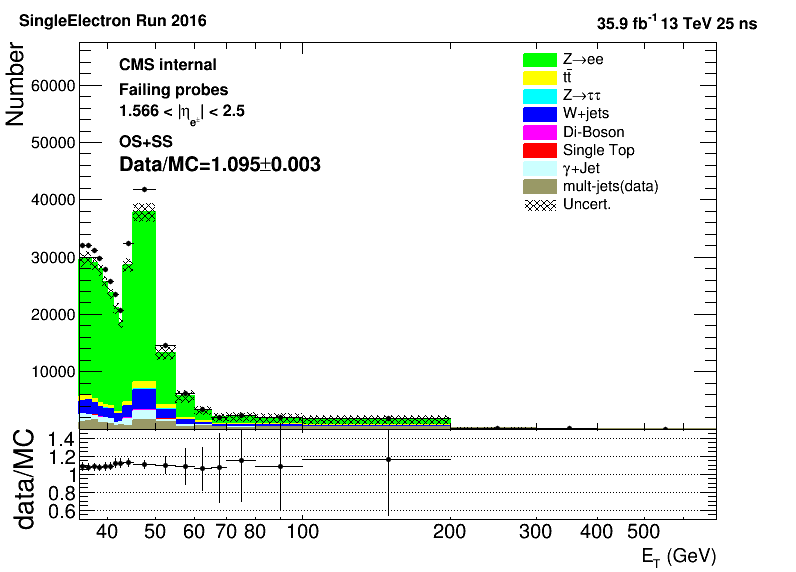
\includegraphics[width=0.45\textwidth]{figures/Zprime/2016/ScaleFactor/SameSign/nominal/stack_Et_Endcap_fail_PUW.png}
    \end{tabular}
    \caption{$E_{T}$ of probe in the barrel (left) and endcap (right) where all the probes are included (top), only passing probes are included (middle) and only failed probes are included (bottom) for 2016.}
    \label{fig:SS_nominal_Et_2016}
  \end{center}
\end{figure}
\begin{figure}[htp]
  \begin{center}
    \begin{tabular}{cc}
      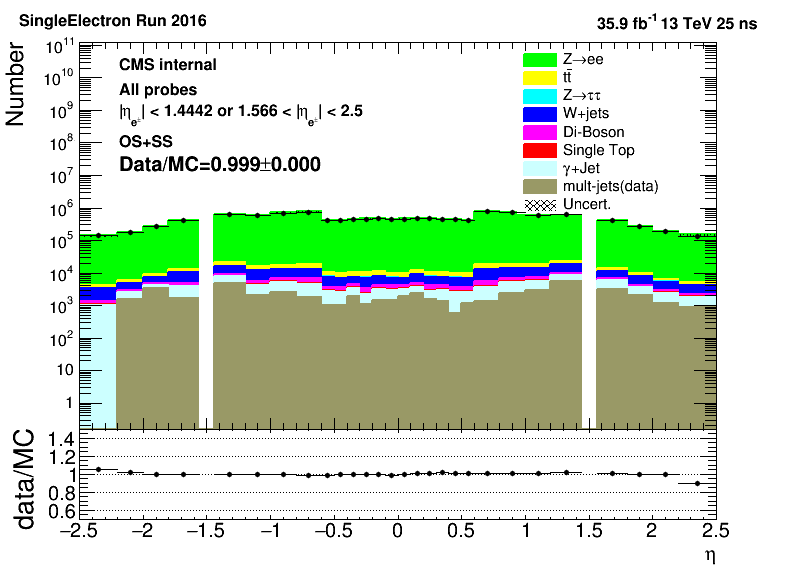
\includegraphics[width=0.45\textwidth]{figures/Zprime/2016/ScaleFactor/SameSign/nominal/stack_eta_BE_Barrel+Endcap_probes_PUW.png} &
      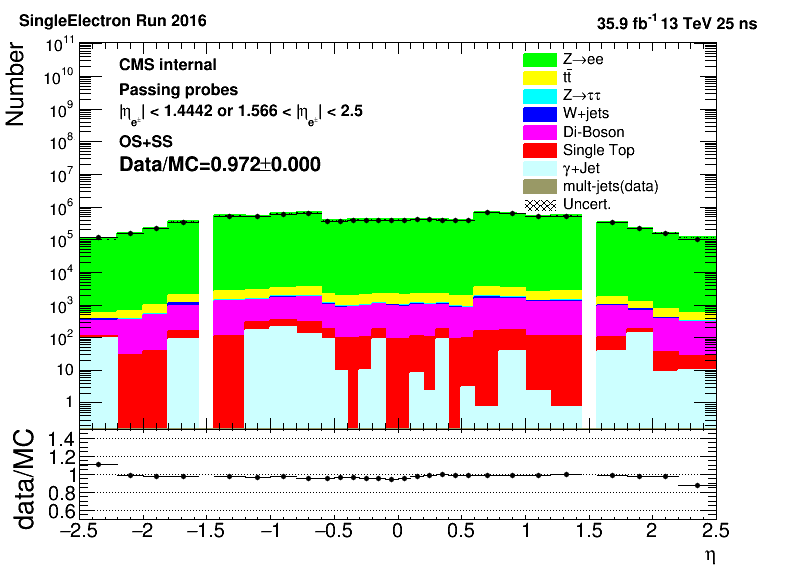
\includegraphics[width=0.45\textwidth]{figures/Zprime/2016/ScaleFactor/SameSign/nominal/stack_eta_BE_Barrel+Endcap_pass_PUW.png} \\
      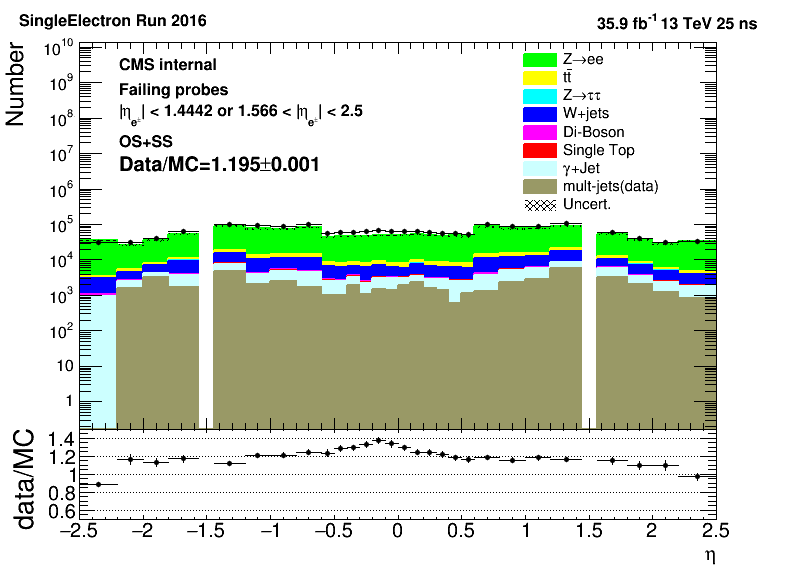
\includegraphics[width=0.45\textwidth]{figures/Zprime/2016/ScaleFactor/SameSign/nominal/stack_eta_BE_Barrel+Endcap_fail_PUW.png} &
    \end{tabular}
    \caption{$\eta$ of probe in the barrel (left) and endcap (right) where all the probes are included (top), only passing probes are included (middle) and only failed probes are included (bottom) for 2016.}
    \label{fig:SS_nominal_eta_2016}
  \end{center}
\end{figure}
\begin{figure}[htp]
  \begin{center}
    \begin{tabular}{cc}
      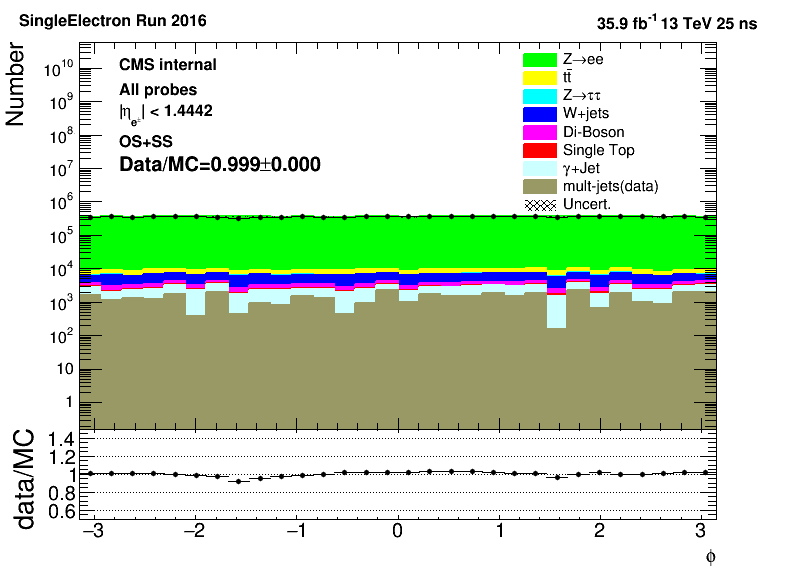
\includegraphics[width=0.45\textwidth]{figures/Zprime/2016/ScaleFactor/SameSign/nominal/stack_phi_Barrel_probes_PUW.png} &
      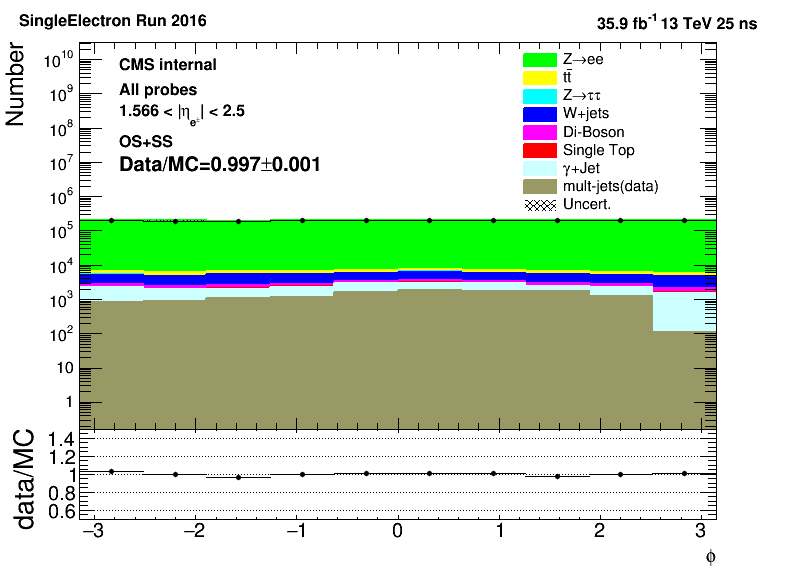
\includegraphics[width=0.45\textwidth]{figures/Zprime/2016/ScaleFactor/SameSign/nominal/stack_phi_Endcap_probes_PUW.png} \\
      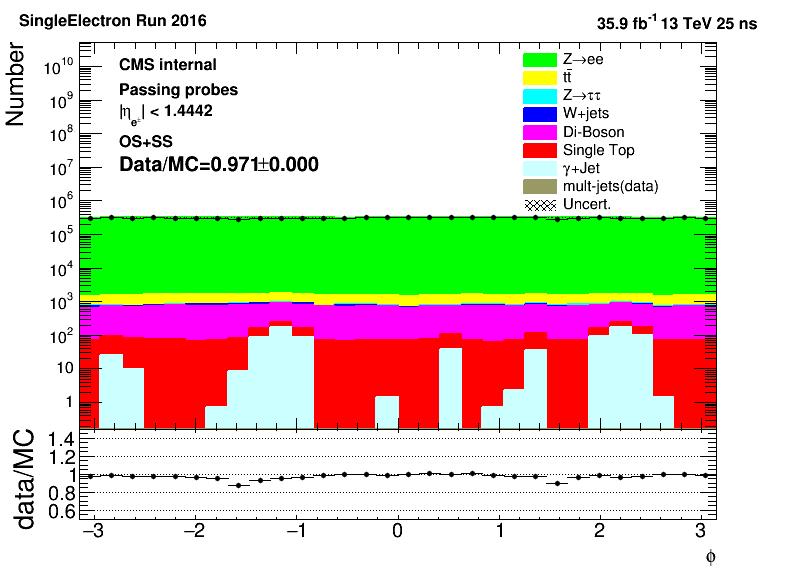
\includegraphics[width=0.45\textwidth]{figures/Zprime/2016/ScaleFactor/SameSign/nominal/stack_phi_Barrel_pass_PUW.png} &
      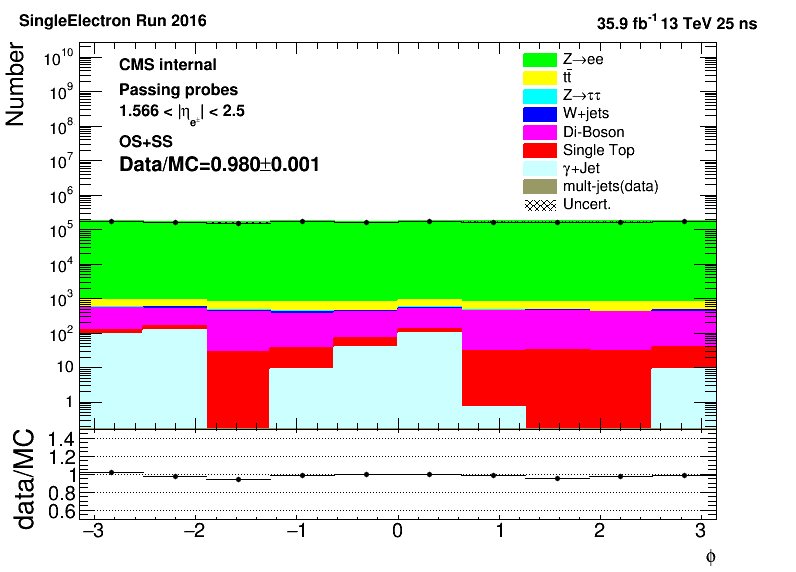
\includegraphics[width=0.45\textwidth]{figures/Zprime/2016/ScaleFactor/SameSign/nominal/stack_phi_Endcap_pass_PUW.png}\\
      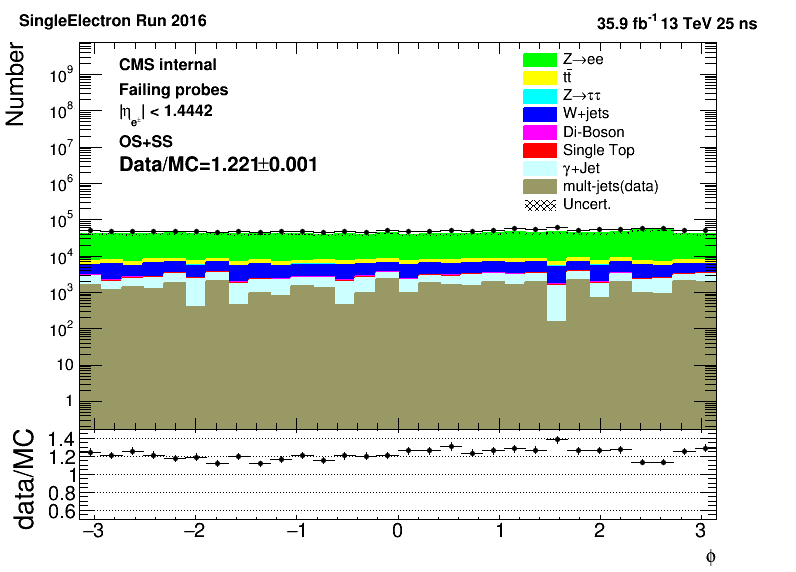
\includegraphics[width=0.45\textwidth]{figures/Zprime/2016/ScaleFactor/SameSign/nominal/stack_phi_Barrel_fail_PUW.png} &
      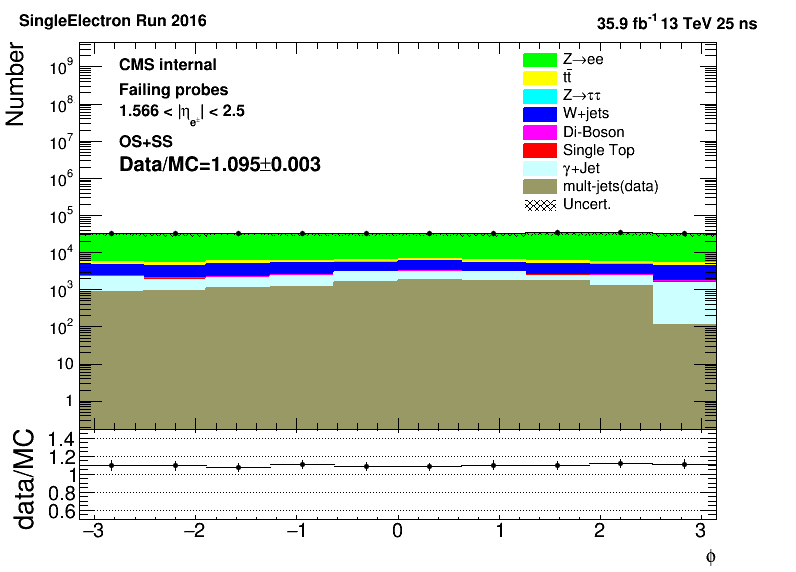
\includegraphics[width=0.45\textwidth]{figures/Zprime/2016/ScaleFactor/SameSign/nominal/stack_phi_Endcap_fail_PUW.png}
    \end{tabular}
    \caption{$\phi$ of probe in the barrel (left) and endcap (right) where all the probes are included (top), only passing probes are included (middle) and only failed probes are included (bottom) for 2016.}
    \label{fig:SS_nominal_phi_2016}
  \end{center}
\end{figure}
\begin{figure}[htp]
  \begin{center}
    \begin{tabular}{cc}
      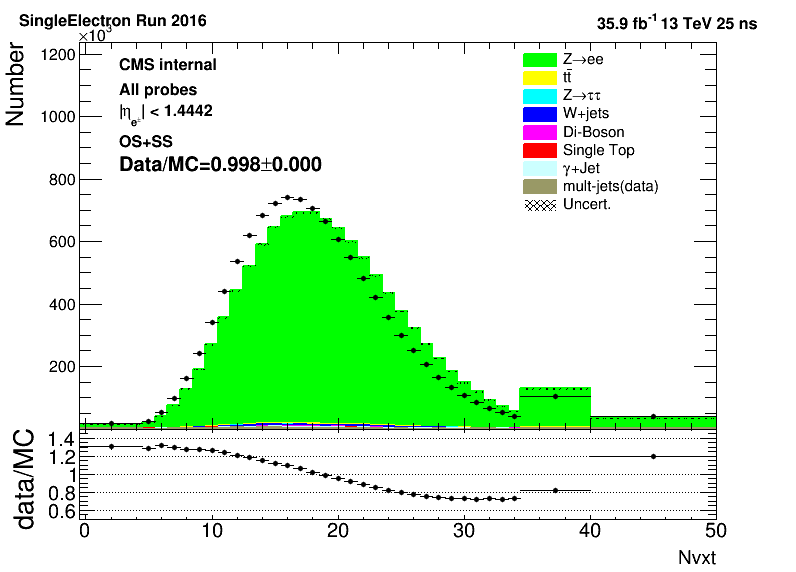
\includegraphics[width=0.45\textwidth]{figures/Zprime/2016/ScaleFactor/SameSign/nominal/stack_nVtx_Barrel_probes_PUW.png} &
      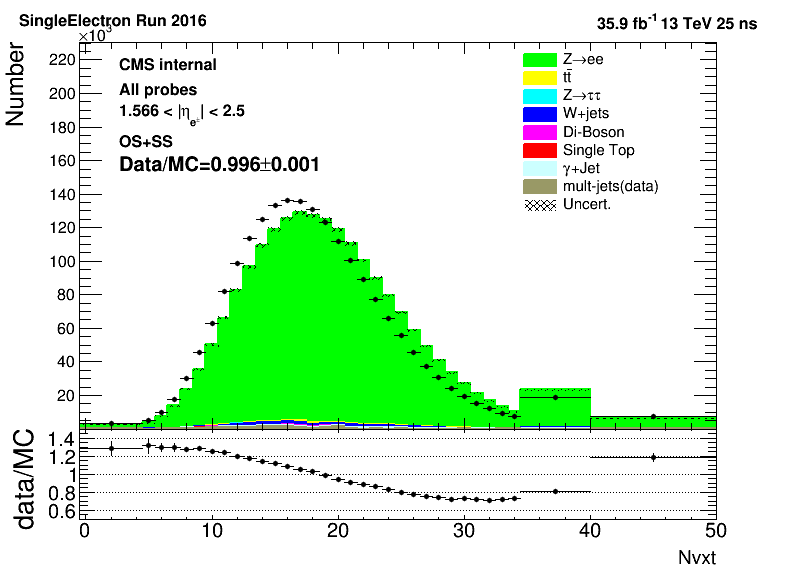
\includegraphics[width=0.45\textwidth]{figures/Zprime/2016/ScaleFactor/SameSign/nominal/stack_nVtx_Endcap_probes_PUW.png} \\
      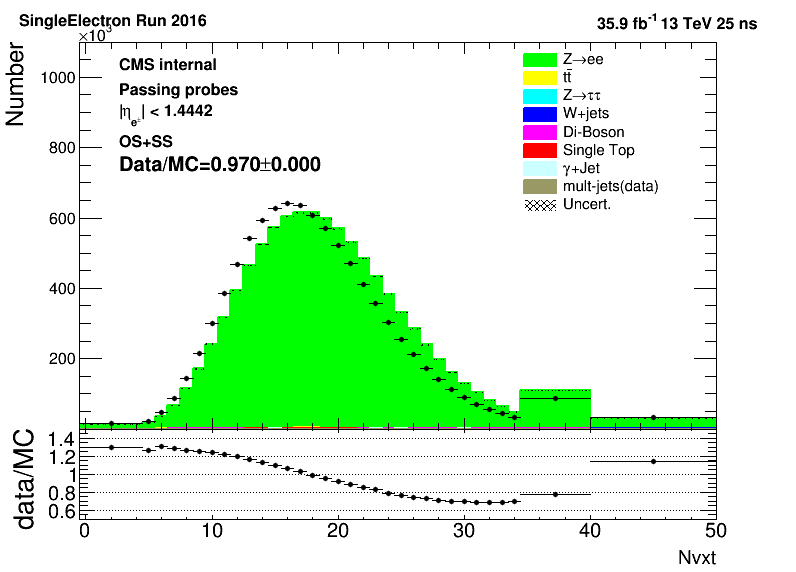
\includegraphics[width=0.45\textwidth]{figures/Zprime/2016/ScaleFactor/SameSign/nominal/stack_nVtx_Barrel_pass_PUW.png} &
      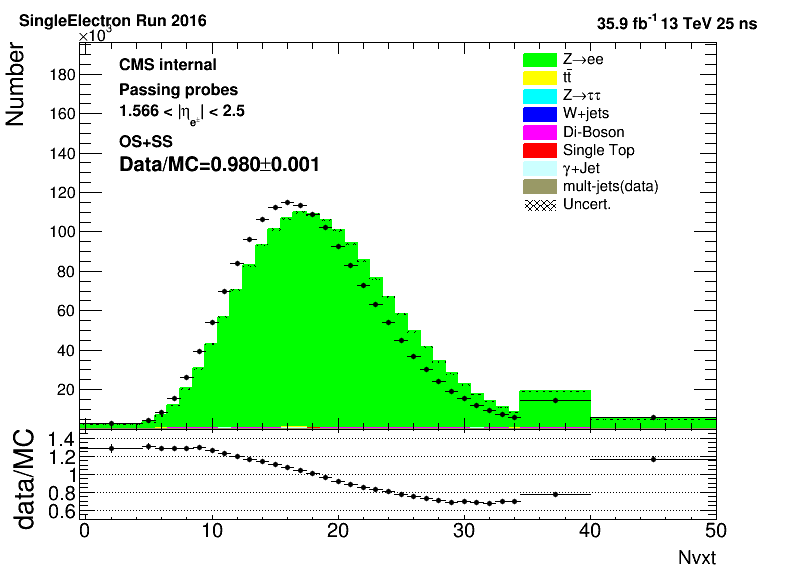
\includegraphics[width=0.45\textwidth]{figures/Zprime/2016/ScaleFactor/SameSign/nominal/stack_nVtx_Endcap_pass_PUW.png}\\
      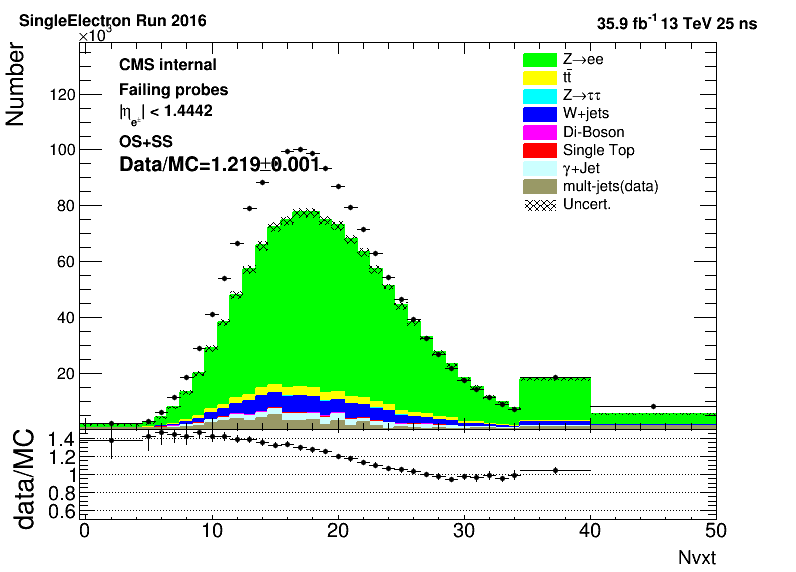
\includegraphics[width=0.45\textwidth]{figures/Zprime/2016/ScaleFactor/SameSign/nominal/stack_nVtx_Barrel_fail_PUW.png} &
      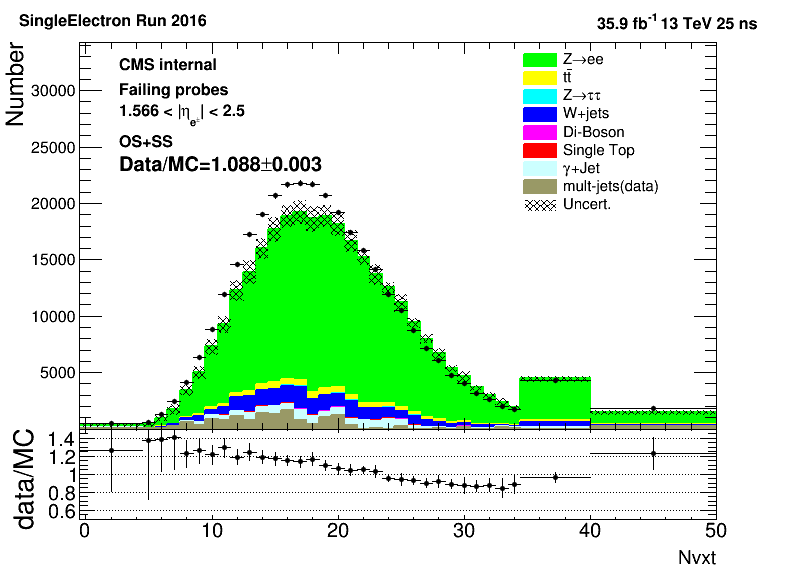
\includegraphics[width=0.45\textwidth]{figures/Zprime/2016/ScaleFactor/SameSign/nominal/stack_nVtx_Endcap_fail_PUW.png}
    \end{tabular}
    \caption{Number of primary vertex of tag and probe pair event in the barrel (left) and endcap (right) where all the probes are included (top), only passing probes are included (middle) and only failed probes are included (bottom) for 2016.}
    \label{fig:SS_nominal_PV_2016}
  \end{center}
\end{figure}



\begin{figure}[htp]
  \begin{center}
    \begin{tabular}{cc}
      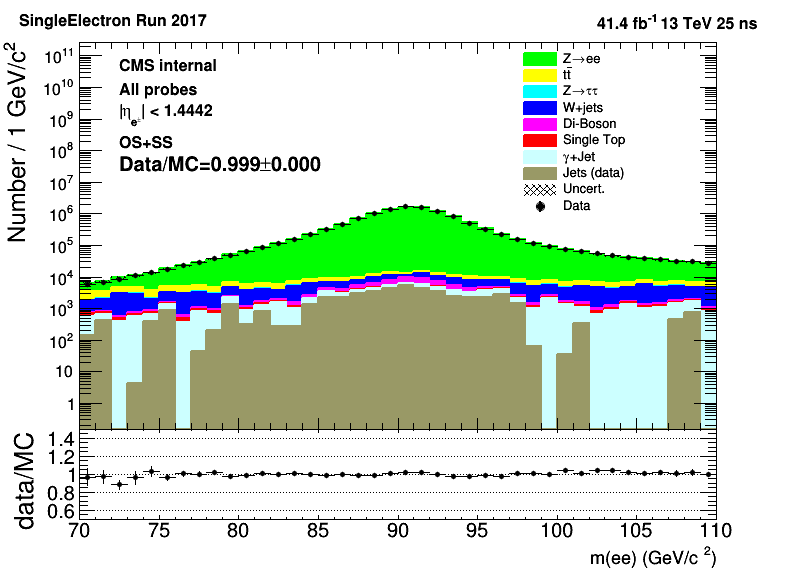
\includegraphics[width=0.45\textwidth]{figures/Zprime/2017/ScaleFactor/SameSign/nominal/stack_mee_Barrel_probes_PUW.png} &
      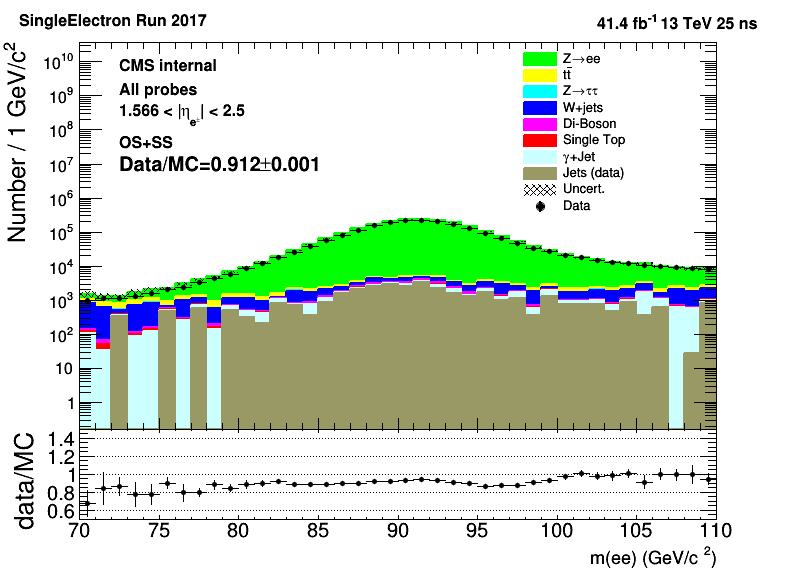
\includegraphics[width=0.45\textwidth]{figures/Zprime/2017/ScaleFactor/SameSign/nominal/stack_mee_Endcap_probes_PUW.png} \\
      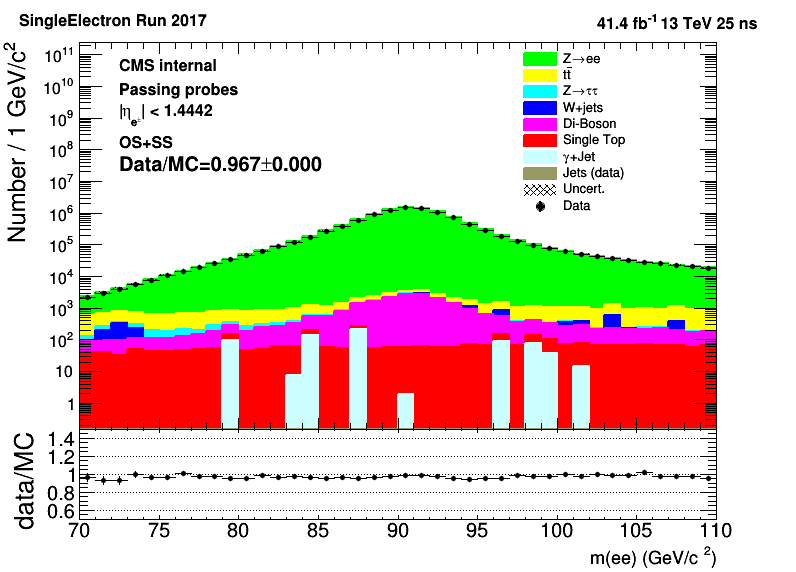
\includegraphics[width=0.45\textwidth]{figures/Zprime/2017/ScaleFactor/SameSign/nominal/stack_mee_Barrel_pass_PUW.png} &
      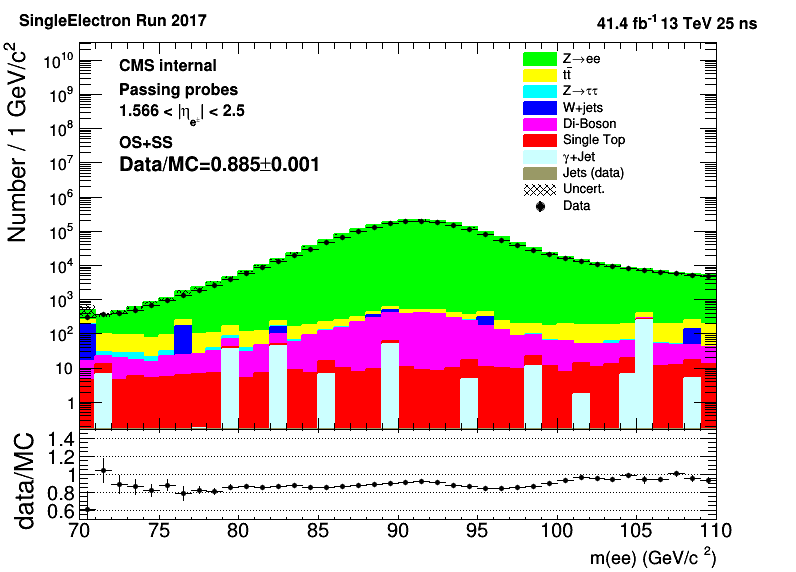
\includegraphics[width=0.45\textwidth]{figures/Zprime/2017/ScaleFactor/SameSign/nominal/stack_mee_Endcap_pass_PUW.png}\\
      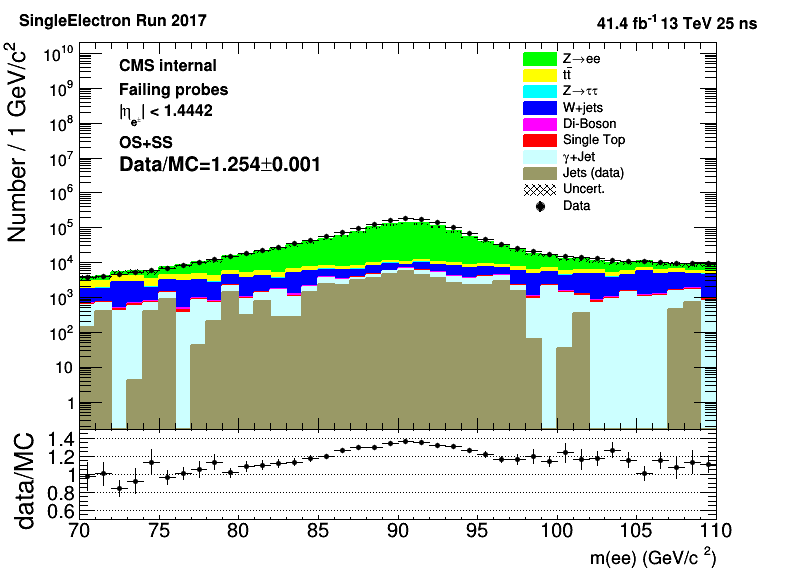
\includegraphics[width=0.45\textwidth]{figures/Zprime/2017/ScaleFactor/SameSign/nominal/stack_mee_Barrel_fail_PUW.png} &
      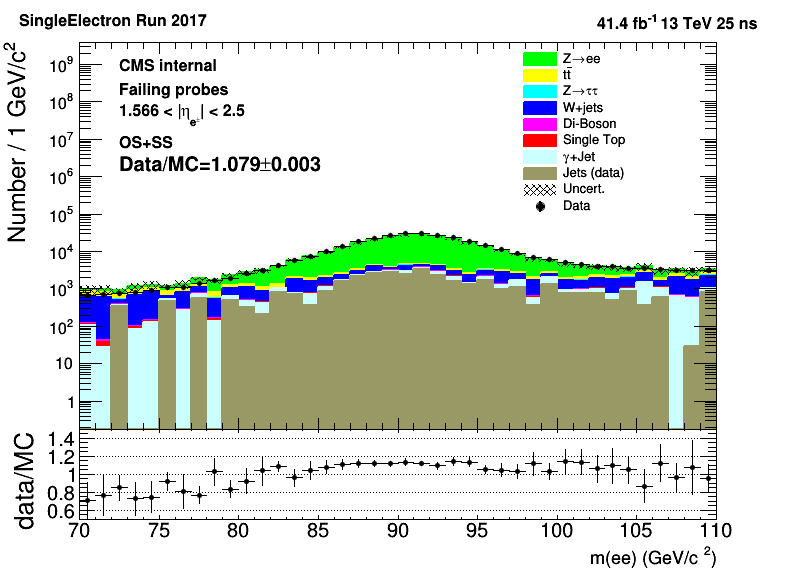
\includegraphics[width=0.45\textwidth]{figures/Zprime/2017/ScaleFactor/SameSign/nominal/stack_mee_Endcap_fail_PUW.png}
    \end{tabular}
    \caption{Invariant mass of tag and probe for probe in the barrel (left) and endcap (right) where all the probes are included (top), only passing probes are included (middle) and only failed probes are included (bottom) for 2017.}
    \label{fig:SS_nominal_mee_2017}
  \end{center}
\end{figure}
\begin{figure}[htp]
  \begin{center}
    \begin{tabular}{cc}
      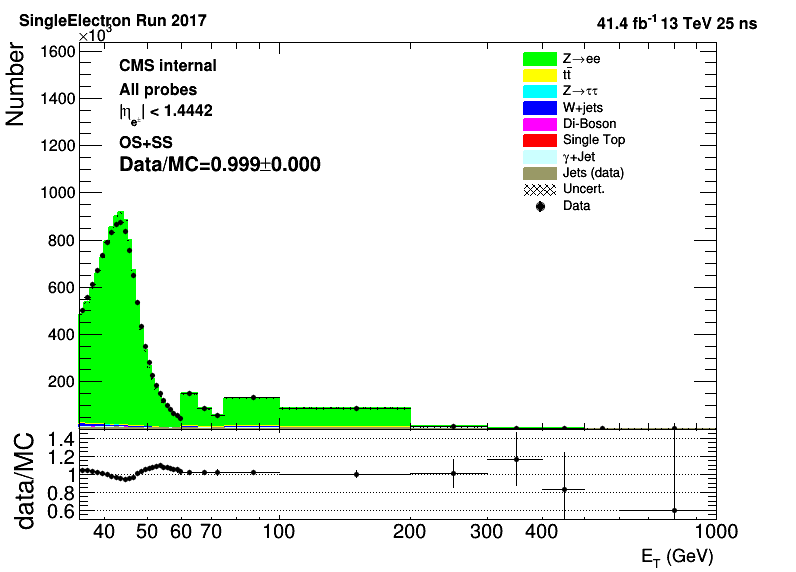
\includegraphics[width=0.45\textwidth]{figures/Zprime/2017/ScaleFactor/SameSign/nominal/stack_Et_Barrel_probes_PUW.png} &
      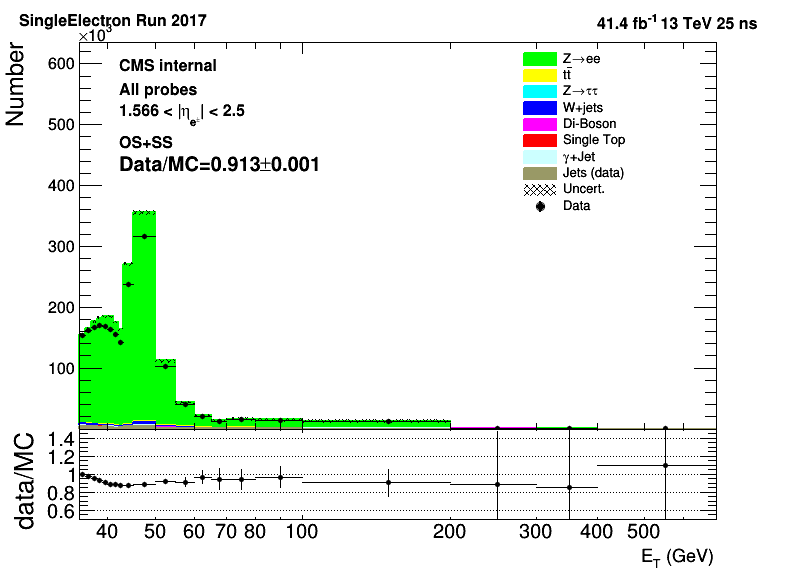
\includegraphics[width=0.45\textwidth]{figures/Zprime/2017/ScaleFactor/SameSign/nominal/stack_Et_Endcap_probes_PUW.png} \\
      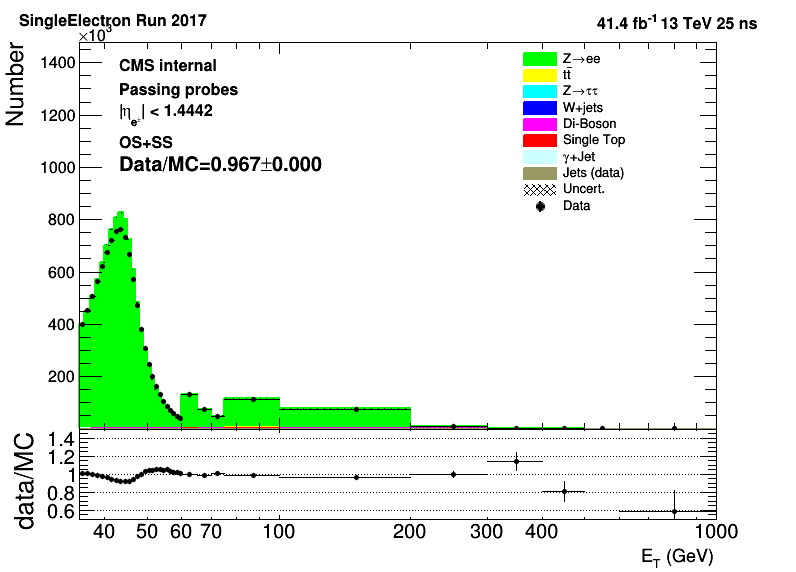
\includegraphics[width=0.45\textwidth]{figures/Zprime/2017/ScaleFactor/SameSign/nominal/stack_Et_Barrel_pass_PUW.png} &
      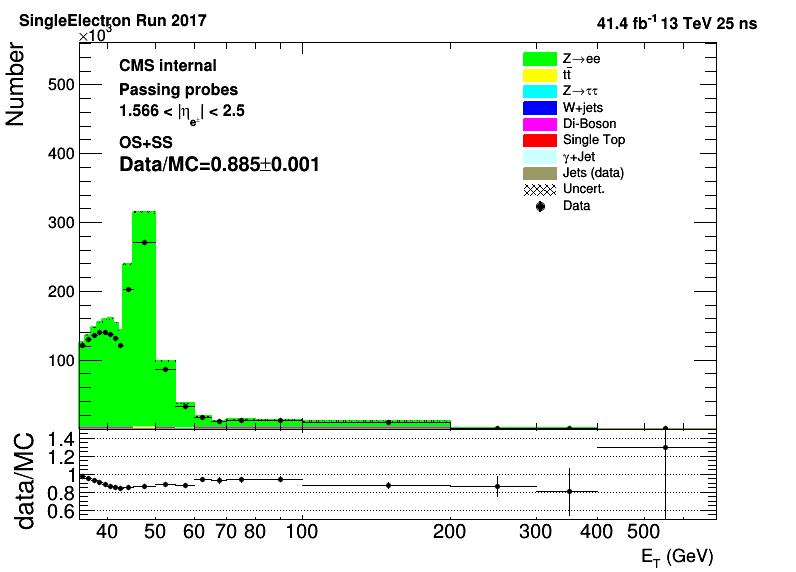
\includegraphics[width=0.45\textwidth]{figures/Zprime/2017/ScaleFactor/SameSign/nominal/stack_Et_Endcap_pass_PUW.png}\\
      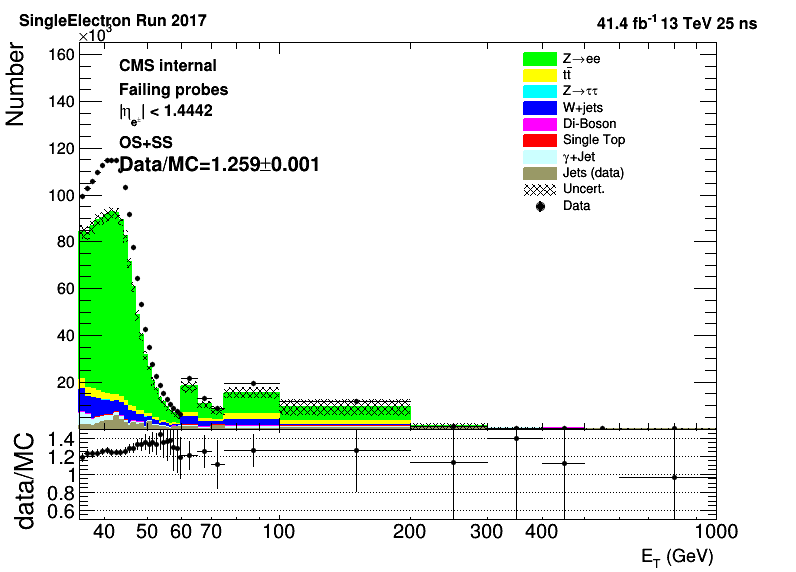
\includegraphics[width=0.45\textwidth]{figures/Zprime/2017/ScaleFactor/SameSign/nominal/stack_Et_Barrel_fail_PUW.png} &
      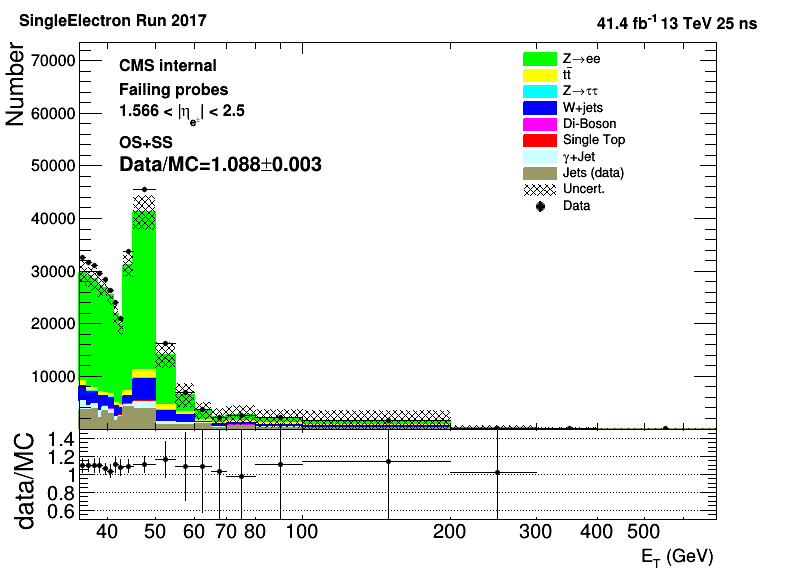
\includegraphics[width=0.45\textwidth]{figures/Zprime/2017/ScaleFactor/SameSign/nominal/stack_Et_Endcap_fail_PUW.png}
    \end{tabular}
    \caption{$E_{T}$ of probe in the barrel (left) and endcap (right) where all the probes are included (top), only passing probes are included (middle) and only failed probes are included (bottom) for 2017.}
    \label{fig:SS_nominal_Et_2017}
  \end{center}
\end{figure}
\begin{figure}[htp]
  \begin{center}
    \begin{tabular}{cc}
      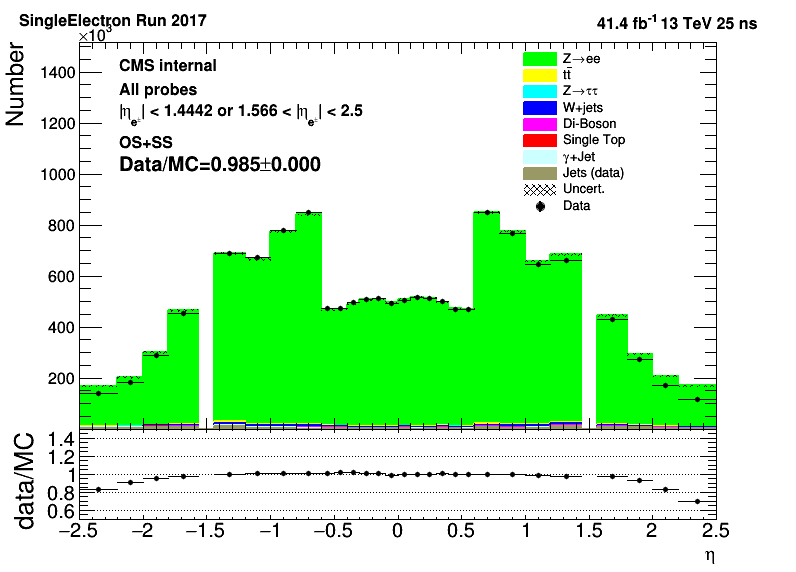
\includegraphics[width=0.45\textwidth]{figures/Zprime/2017/ScaleFactor/SameSign/nominal/stack_eta_BE_Barrel+Endcap_probes_PUW.png} &
      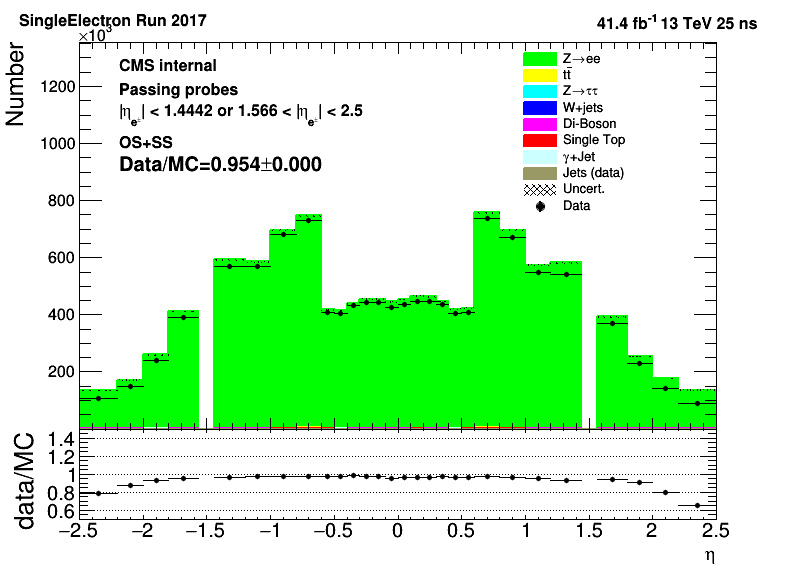
\includegraphics[width=0.45\textwidth]{figures/Zprime/2017/ScaleFactor/SameSign/nominal/stack_eta_BE_Barrel+Endcap_pass_PUW.png} \\
      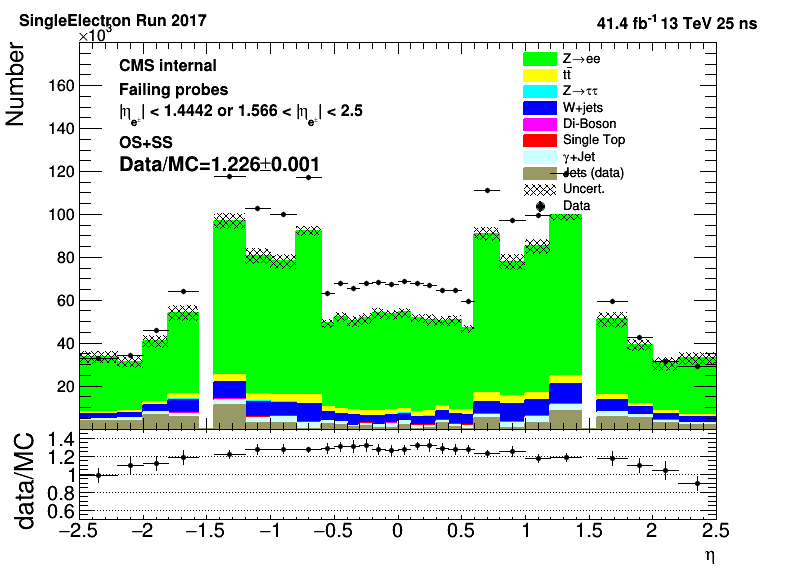
\includegraphics[width=0.45\textwidth]{figures/Zprime/2017/ScaleFactor/SameSign/nominal/stack_eta_BE_Barrel+Endcap_fail_PUW.png} &
    \end{tabular}
    \caption{$\eta$ of probe in the barrel (left) and endcap (right) where all the probes are included (top), only passing probes are included (middle) and only failed probes are included (bottom) for 2017.}
    \label{fig:SS_nominal_eta_2017}
  \end{center}
\end{figure}
\begin{figure}[htp]
  \begin{center}
    \begin{tabular}{cc}
      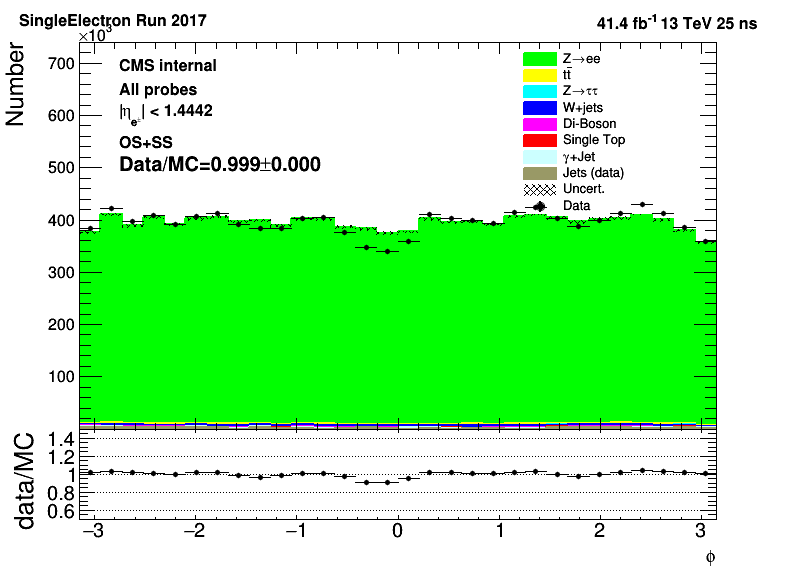
\includegraphics[width=0.45\textwidth]{figures/Zprime/2017/ScaleFactor/SameSign/nominal/stack_phi_Barrel_probes_PUW.png} &
      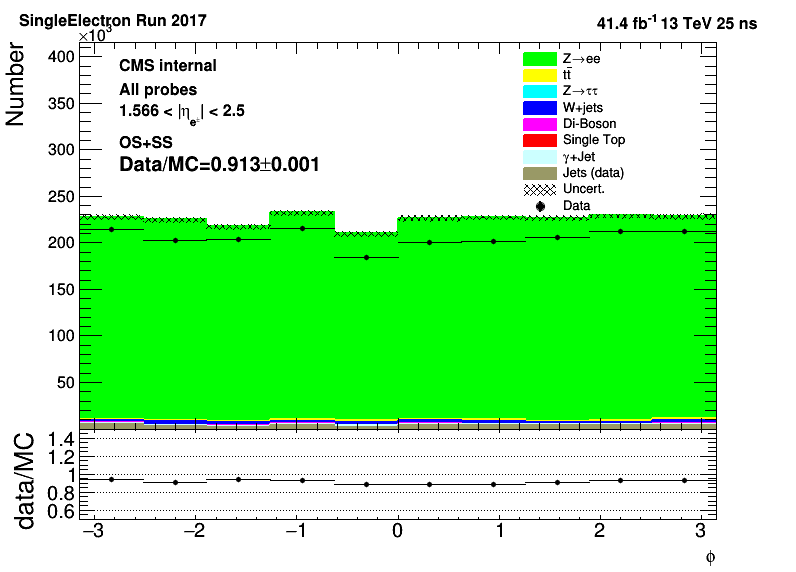
\includegraphics[width=0.45\textwidth]{figures/Zprime/2017/ScaleFactor/SameSign/nominal/stack_phi_Endcap_probes_PUW.png} \\
      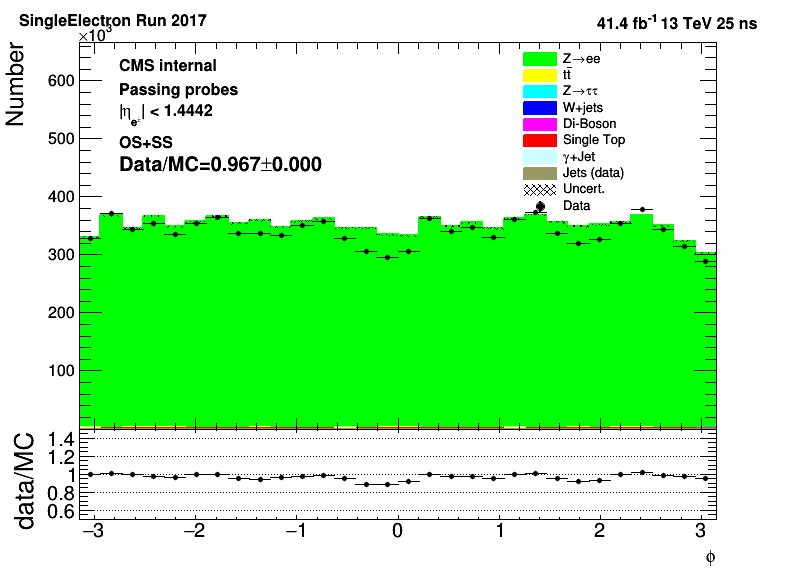
\includegraphics[width=0.45\textwidth]{figures/Zprime/2017/ScaleFactor/SameSign/nominal/stack_phi_Barrel_pass_PUW.png} &
      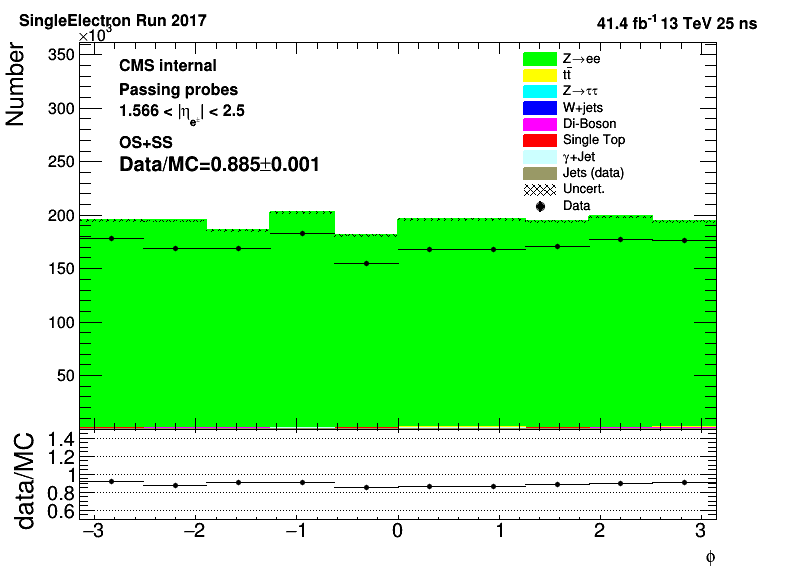
\includegraphics[width=0.45\textwidth]{figures/Zprime/2017/ScaleFactor/SameSign/nominal/stack_phi_Endcap_pass_PUW.png}\\
      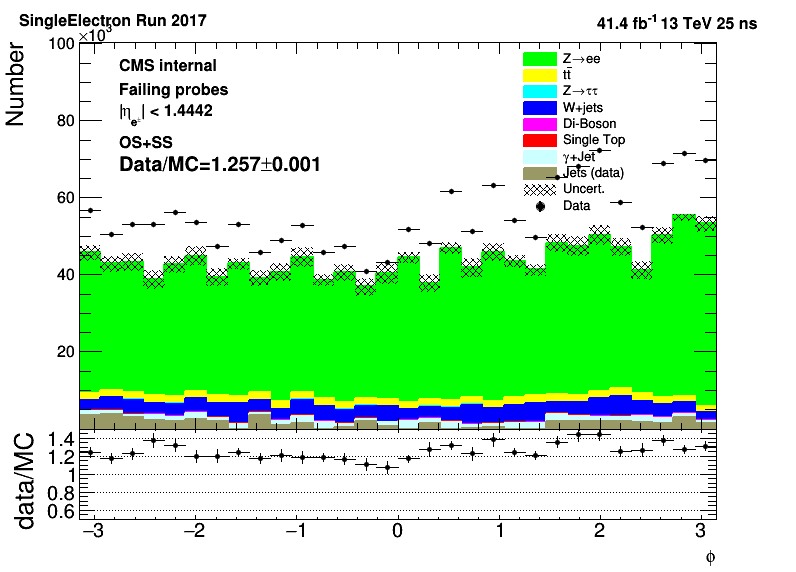
\includegraphics[width=0.45\textwidth]{figures/Zprime/2017/ScaleFactor/SameSign/nominal/stack_phi_Barrel_fail_PUW.png} &
      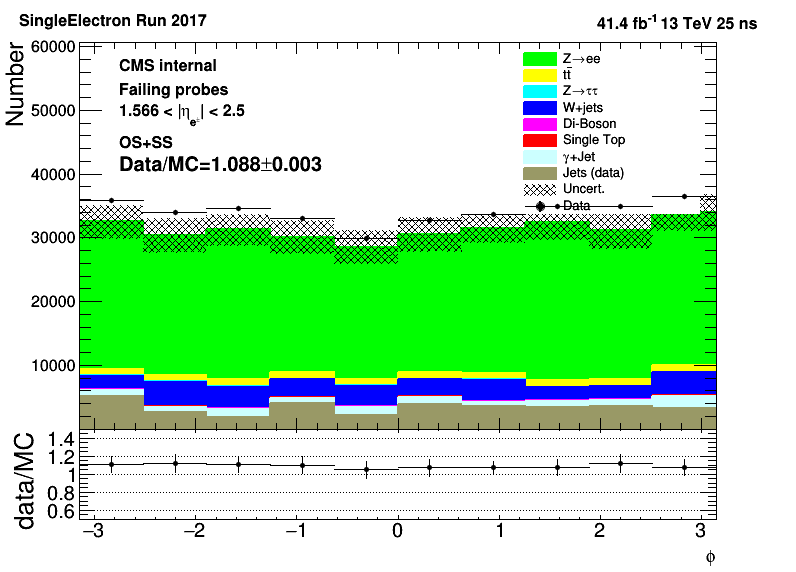
\includegraphics[width=0.45\textwidth]{figures/Zprime/2017/ScaleFactor/SameSign/nominal/stack_phi_Endcap_fail_PUW.png}
    \end{tabular}
    \caption{$\phi$ of probe in the barrel (left) and endcap (right) where all the probes are included (top), only passing probes are included (middle) and only failed probes are included (bottom) for 2017.}
    \label{fig:SS_nominal_phi_2017}
  \end{center}
\end{figure}
\begin{figure}[htp]
  \begin{center}
    \begin{tabular}{cc}
      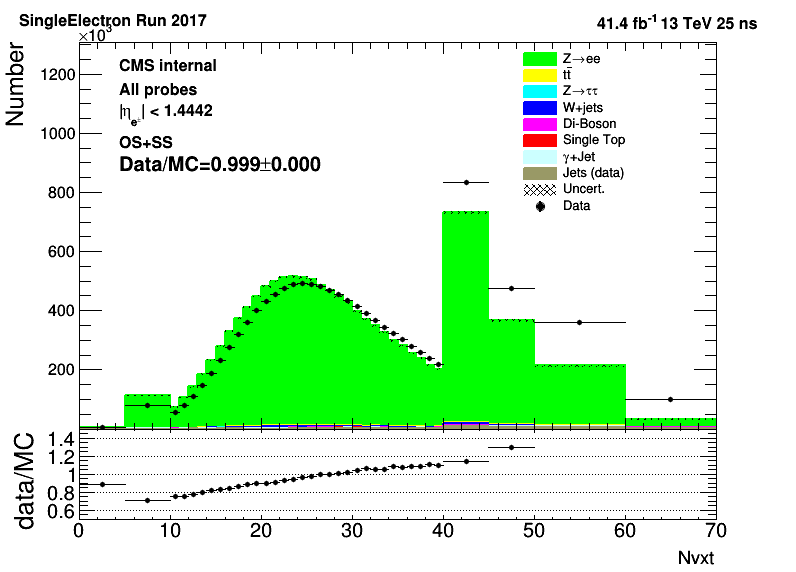
\includegraphics[width=0.45\textwidth]{figures/Zprime/2017/ScaleFactor/SameSign/nominal/stack_nVtx_Barrel_probes_PUW.png} &
      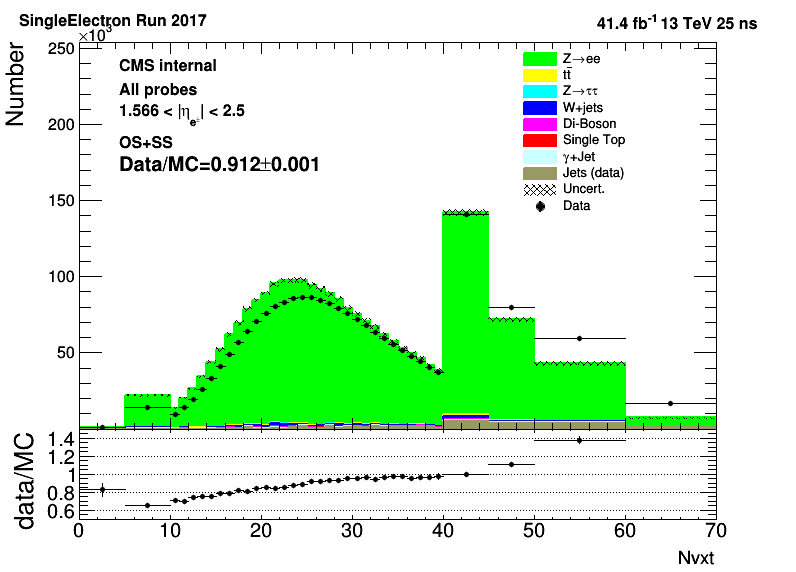
\includegraphics[width=0.45\textwidth]{figures/Zprime/2017/ScaleFactor/SameSign/nominal/stack_nVtx_Endcap_probes_PUW.png} \\
      \includegraphics[width=0.45\textwidth]{figures/Zprime/2017/ScaleFactor/SameSign/nominal/stack_nVtx_Barrel_pass_PUW.png} &
      \includegraphics[width=0.45\textwidth]{figures/Zprime/2017/ScaleFactor/SameSign/nominal/stack_nVtx_Endcap_pass_PUW.png}\\
      \includegraphics[width=0.45\textwidth]{figures/Zprime/2017/ScaleFactor/SameSign/nominal/stack_nVtx_Barrel_fail_PUW.png} &
      \includegraphics[width=0.45\textwidth]{figures/Zprime/2017/ScaleFactor/SameSign/nominal/stack_nVtx_Endcap_fail_PUW.png}
    \end{tabular}
    \caption{Number of primary vertex of tag and probe pair event in the barrel (left) and endcap (right) where all the probes are included (top), only passing probes are included (middle) and only failed probes are included (bottom) for 2017.}
    \label{fig:SS_nominal_PV_2017}
  \end{center}
\end{figure}

\clearpage
\subsection{HEEP ID efficiencies and scale factors}
\label{subsubsec:SF_results}
In 2016 the HEEP ID efficiencies for data and MC are shown as functions of $E_T$, $\eta$, and $\phi$ of the probe, and of $N_{vtx}$ in figures \ref{fig:eff_SS_nominal_ET_2016}-\ref{fig:eff_SS_nominal_nVtx_2016} (left), here data includes both DY and non-DY events. In order to check if the contribution of non-DY backgrounds are estimated correctly, the DY efficiency is compared to data while non-DY contributions are subtracted from data in figures \ref{fig:eff_SS_nominal_ET_2016}-\ref{fig:eff_SS_nominal_nVtx_2016} (right). The scale factors obtained with these two approaches are in a good agreement in all variables. In addition, data to MC scale factor per bin and the mean value are shown in the bottom pad of the same plot.
Same plots in 2017 are shown in figures \ref{fig:eff_SS_nominal_ET_2017}-\ref{fig:eff_SS_nominal_nVtx_2017}.
\begin{figure}[htp]
  \begin{center}
    \begin{tabular}{cc}
      \includegraphics[width=0.45\textwidth]{figures/Zprime/2016/ScaleFactor/SameSign/nominal/g_compare_cut_Et_Barrel_ea_ta_inc_AS_nominal_PUW.png} &
      \includegraphics[width=0.45\textwidth]{figures/Zprime/2016/ScaleFactor/SameSign/nominal/g_compare_cut_Et_Barrel_ea_ta_exc_AS_nominal_PUW.png} \\
      \includegraphics[width=0.45\textwidth]{figures/Zprime/2016/ScaleFactor/SameSign/nominal/g_compare_cut_Et_Endcap_ea_ta_inc_AS_nominal_PUW.png} &
      \includegraphics[width=0.45\textwidth]{figures/Zprime/2016/ScaleFactor/SameSign/nominal/g_compare_cut_Et_Endcap_ea_ta_exc_AS_nominal_PUW.png}
    \end{tabular}
    \caption{Efficiencies and scale factors in MC and data in the barrel (top) and endcap (bottom) where the non-DY processes are included (left) and subtracted (right) as functions of probe $E_T$ in 2016.}
    \label{fig:eff_SS_nominal_ET_2016}
  \end{center}
\end{figure}

\begin{figure}[htp]
  \begin{center}
    \begin{tabular}{cc}
      \includegraphics[width=0.45\textwidth]{figures/Zprime/2016/ScaleFactor/SameSign/nominal/g_compare_cut_eta_Barrel+Endcap_ea_ta_inc_AS_nominal_PUW.png} &
      \includegraphics[width=0.45\textwidth]{figures/Zprime/2016/ScaleFactor/SameSign/nominal/g_compare_cut_eta_Barrel+Endcap_ea_ta_exc_AS_nominal_PUW.png} \\
    \end{tabular}
    \caption{Efficiencies and scale factors in MC and data where the non-DY processes are included (left) and subtracted (right) as functions of probe $\eta$ in 2016.}
    \label{fig:eff_SS_nominal_eta_2016}
  \end{center}
\end{figure}

\begin{figure}[htp]
  \begin{center}
    \begin{tabular}{cc}
      \includegraphics[width=0.45\textwidth,height=6.3cm]{figures/Zprime/2016/ScaleFactor/SameSign/nominal/g_compare_cut_phi_Barrel_ea_ta_inc_AS_nominal_PUW.png} &
      \includegraphics[width=0.45\textwidth,height=6.3cm]{figures/Zprime/2016/ScaleFactor/SameSign/nominal/g_compare_cut_phi_Barrel_ea_ta_exc_AS_nominal_PUW.png} \\
      \includegraphics[width=0.45\textwidth,height=6.3cm]{figures/Zprime/2016/ScaleFactor/SameSign/nominal/g_compare_cut_phi_Endcap_ea_ta_inc_AS_nominal_PUW.png} &
      \includegraphics[width=0.45\textwidth,height=6.3cm]{figures/Zprime/2016/ScaleFactor/SameSign/nominal/g_compare_cut_phi_Endcap_ea_ta_exc_AS_nominal_PUW.png}
    \end{tabular}
    \caption{Efficiencies and scale factors in MC and data in the barrel (top) and endcap (bottom) where the non-DY processes are included (left) and subtracted (right) as functions of probe $\phi$ in 2016.}
    \label{fig:eff_SS_nominal_phi_2016}
  \end{center}
\end{figure}

\begin{figure}[bh]
  \begin{center}
    \begin{tabular}{cc}
      \includegraphics[width=0.45\textwidth]{figures/Zprime/2016/ScaleFactor/SameSign/nominal/g_compare_cut_nVtx_Barrel_ea_ta_inc_AS_nominal_PUW.png} &
      \includegraphics[width=0.45\textwidth]{figures/Zprime/2016/ScaleFactor/SameSign/nominal/g_compare_cut_nVtx_Barrel_ea_ta_exc_AS_nominal_PUW.png} \\
      \includegraphics[width=0.45\textwidth]{figures/Zprime/2016/ScaleFactor/SameSign/nominal/g_compare_cut_nVtx_Endcap_ea_ta_inc_AS_nominal_PUW.png} &
      \includegraphics[width=0.45\textwidth]{figures/Zprime/2016/ScaleFactor/SameSign/nominal/g_compare_cut_nVtx_Endcap_ea_ta_exc_AS_nominal_PUW.png}
    \end{tabular}
    \caption{Efficiencies and scale factors in MC and data in the barrel (top) and endcap (bottom) where the non-DY processes are included (left) and subtracted (right) as functions of the number of primary vertices, $n_{Vtx}$ in 2016.}
    \label{fig:eff_SS_nominal_nVtx_2016}
  \end{center}
\end{figure}


\begin{figure}[htp]
  \begin{center}
    \begin{tabular}{cc}
      \includegraphics[width=0.45\textwidth]{figures/Zprime/2017/ScaleFactor/SameSign/nominal/g_compare_cut_Et_Barrel_ea_ta_inc_AS_nominal_PUW.png} &
      \includegraphics[width=0.45\textwidth]{figures/Zprime/2017/ScaleFactor/SameSign/nominal/g_compare_cut_Et_Barrel_ea_ta_exc_AS_nominal_PUW.png} \\
      \includegraphics[width=0.45\textwidth]{figures/Zprime/2017/ScaleFactor/SameSign/nominal/g_compare_cut_Et_Endcap_ea_ta_inc_AS_nominal_PUW.png} &
      \includegraphics[width=0.45\textwidth]{figures/Zprime/2017/ScaleFactor/SameSign/nominal/g_compare_cut_Et_Endcap_ea_ta_exc_AS_nominal_PUW.png}
    \end{tabular}
    \caption{Efficiencies and scale factors in MC and data in the barrel (top) and endcap (bottom) where the non-DY processes are included (left) and subtracted (right) as functions of probe $E_T$ in 2017.}
    \label{fig:eff_SS_nominal_ET_2017}
  \end{center}
\end{figure}

\begin{figure}[htp]
  \begin{center}
    \begin{tabular}{cc}
      \includegraphics[width=0.45\textwidth]{figures/Zprime/2017/ScaleFactor/SameSign/nominal/g_compare_cut_eta_Barrel+Endcap_ea_ta_inc_AS_nominal_PUW.png} &
      \includegraphics[width=0.45\textwidth]{figures/Zprime/2017/ScaleFactor/SameSign/nominal/g_compare_cut_eta_Barrel+Endcap_ea_ta_exc_AS_nominal_PUW.png} \\
    \end{tabular}
    \caption{Efficiencies and scale factors in MC and data where the non-DY processes are included (left) and subtracted (right) as functions of probe $\eta$ in 2017.}
    \label{fig:eff_SS_nominal_eta_2017}
  \end{center}
\end{figure}

\begin{figure}[htp]
  \begin{center}
    \begin{tabular}{cc}
      \includegraphics[width=0.45\textwidth,height=6.3cm]{figures/Zprime/2017/ScaleFactor/SameSign/nominal/g_compare_cut_phi_Barrel_ea_ta_inc_AS_nominal_PUW.png} &
      \includegraphics[width=0.45\textwidth,height=6.3cm]{figures/Zprime/2017/ScaleFactor/SameSign/nominal/g_compare_cut_phi_Barrel_ea_ta_exc_AS_nominal_PUW.png} \\
      \includegraphics[width=0.45\textwidth,height=6.3cm]{figures/Zprime/2017/ScaleFactor/SameSign/nominal/g_compare_cut_phi_Endcap_ea_ta_inc_AS_nominal_PUW.png} &
      \includegraphics[width=0.45\textwidth,height=6.3cm]{figures/Zprime/2017/ScaleFactor/SameSign/nominal/g_compare_cut_phi_Endcap_ea_ta_exc_AS_nominal_PUW.png}
    \end{tabular}
    \caption{Efficiencies and scale factors in MC and data in the barrel (top) and endcap (bottom) where the non-DY processes are included (left) and subtracted (right) as functions of probe $\phi$ in 2017.}
    \label{fig:eff_SS_nominal_phi_2017}
  \end{center}
\end{figure}

\begin{figure}[bh]
  \begin{center}
    \begin{tabular}{cc}
      \includegraphics[width=0.45\textwidth]{figures/Zprime/2017/ScaleFactor/SameSign/nominal/g_compare_cut_nVtx_Barrel_ea_ta_inc_AS_nominal_PUW.png} &
      \includegraphics[width=0.45\textwidth]{figures/Zprime/2017/ScaleFactor/SameSign/nominal/g_compare_cut_nVtx_Barrel_ea_ta_exc_AS_nominal_PUW.png} \\
      \includegraphics[width=0.45\textwidth]{figures/Zprime/2017/ScaleFactor/SameSign/nominal/g_compare_cut_nVtx_Endcap_ea_ta_inc_AS_nominal_PUW.png} &
      \includegraphics[width=0.45\textwidth]{figures/Zprime/2017/ScaleFactor/SameSign/nominal/g_compare_cut_nVtx_Endcap_ea_ta_exc_AS_nominal_PUW.png}
    \end{tabular}
    \caption{Efficiencies and scale factors in MC and data in the barrel (top) and endcap (bottom) where the non-DY processes are included (left) and subtracted (right) as functions of the number of primary vertices, $n_{Vtx}$ in 2017.}
    \label{fig:eff_SS_nominal_nVtx_2017}
  \end{center}
\end{figure}

\clearpage

The main sources of systematic uncertainties on the scale factor originate from non-DY processes.
The nominal value of the cross sections are varied by 10\% and 50\% for $t\bar{t}$ and $W+$jets processes, respectively.
For QCD estimation, we also consider 50\% uncertainty.
%Besides, the uncertainty of the  pileup weights is also considered although it is negligible.
The summary of the efficiencies and scale factors are shown in Table \ref{tab:HEEP_eff_nominal}.

\begin{table}[htp]
  \begin{center}
    \begin{tabular}{|l|l|l|l|}
      \hline
   Year &   & Barrel & Endcap \\ \hline \hline
\multirow{6}{*}{2016} &   Data          & $86.13\% \pm 0.01\%(stat.)$                   & $83.38\% \pm 0.03\%(stat.)$ \\
    &  DY + non-DY   & $88.65\% \pm 0.03\%(stat.)$                   & $84.85\% \pm 0.09\%(stat.)$ \\
    &  Scale factor  & $0.972  \pm 0.000(stat.)\pm 0.006(syst.)$     & $0.983   \pm 0.001(stat.) \pm 0.007(syst.) $ \\ \cline{2-4}
    &  Data - non-DY & $87.92\% \pm 0.03\%(stat.)$                   & $85.83\% \pm 0.09\%(stat.)$ \\
    &  DY            & $90.50\% \pm 0.01\%(stat.)$                   & $87.35\% \pm 0.03\%(stat.)$ \\
    &  Scale factor  & $0.971 \pm 0.000(stat.) \pm 0.006(syst.)$     & $0.983   \pm 0.001(stat.) \pm 0.007(syst.)$ \\
      \hline

\multirow{6}{*}{2017} &     Data          & $86.01\% \pm 0.01\%(stat.)$                   & $83.46\% \pm 0.03\%(stat.)$ \\
     & DY + non-DY   & $88.89\% \pm 0.05\%(stat.)$                   & $86.12\% \pm 0.14\%(stat.)$ \\
     & Scale factor  & $0.968  \pm 0.001(stat.)\pm 0.005(syst.)$     & $0.969   \pm 0.002(stat.)\pm 0.01(syst.)$ \\   \cline{2-4}
     & Data - non-DY & $87.81\% \pm 0.05\%(stat.)$                   & $87.02\% \pm 0.16\%(stat.)$ \\
     & DY            & $90.77\% \pm 0.02\%(stat.)$                   & $89.48\% \pm 0.04\%(stat.)$ \\
     & Scale factor  & $0.967 \pm 0.001(stat.)\pm 0.005(syst.)$      & $0.973   \pm 0.002(stat.)\pm 0.01(syst.)$ \\
      \hline
    \end{tabular}
  \end{center}
  \caption{\label{tab:HEEP_eff_nominal}
  Efficiencies and scale factors in MC and data in the barrel and endcap for non-DY processes included and subtracted.}
\end{table}


It is worth mentioning that many complementary studies are done to understand HEEP scale factor better. Important points are summarized in the following and related plots can be found in Appendix.
\begin{itemize}
  \item[$\bullet$] In 2016
  \item[$\bullet$] the DYToEE Monte Carlo sample used had a special global tag which was discovered late in the process. This tag has a different ECAL noise profile and different transparency corrections which could impact our scale factor. The efficiency vs gen $E_T$ for this inclusive sample was compared to the mass binned samples in figure\ref{fig:eff_ZToEE_DYToEE_ET} and they were found to be similar, with a deviation of only 0.3\% at low $E_T$ in the barrel and up to 1\% in the endcap. It should be noted that the deviation in the endcap will act to flatten the scale factor. Thus it is concluded that impact of the special global tag used in the DYToEE sample does not impact the scale factor measurement significantly.
  \item[$\bullet$] The HEEP scale factor in the last two bins of $E_{T}$ in the endcap seems unusual and DY efficiency is 100\%. The reason could be either a statistical fluctuations or something in Moriond17 MC DY sample. In Appendix \ref{AppHEEPsf_amcatnlo_2016}, we cross checked the HEEP efficiency and scale factor using DYJetsToLL amcatnlo sample which shows the DY efficiency in endcap in last two bins are normal. From figure~\ref{fig:eff_ZToEE_DYToEE_ET}, it can be seen that the efficiency in the MC for 500~GeV electrons is normal if you don't apply the Z constraint and so it is thought to be a statistical fluctuation.
  \item[$\bullet$] HEEP scale factor drops 2\% around $|\eta|=0$. This is mostly related to 'HIP' (Heavy Interacting Particle) problem which means the heavy interacting particle (most are hadron) produced a huge current in silicon strips and make them off for few bunch crossing and we lose hits from electrons. This problem is present in runs B-F and is removed in runs G-H. This issue is discussed in \ref{AppHEEPsf_eta_Et_bins_2016}.
  \item[$\bullet$] there is a turn on effect of scale factor at low $E_{T}$.This comes mainly from shower shape variable (which can be seen in Appendix \ref{AppHEEPsf_N_1_2016} Figure \ref{fig:Shower_2016}). This effect is small (<1\%) so it is ignored.
\end{itemize}
\medskip
\begin{itemize}
  \item[$\circ$] In 2017
  \item[$\circ$] In run F the pixel detector has a lower efficiency in some region which can be seen in Figure \ref{fig:EcalDriven_runF_2017} in Appendix \ref{AppHEEPsf_2017}. This problem causes the lower HEEP ID efficiency in run F.
  \item[$\circ$] The HEEP ID efficiency in data after non-DY contributions are subtracted for different runs for barrel and endcap in 2017 is shown in Figure \ref{fig:Runs_HEEP_eff_rereco_2017}. The efficiency is lower in run B this is because at the beginning of the data taking the detector does not work in very good condition. The efficiency decreases in run E this is because the pile up is significant increased after run E which is shown in Figure \ref{fig:Z_pileup}. Comparing 2016 the average HEEP ID efficiency in barrel is close in 2017, for endcap it is improved in 2017.
  \item[$\circ$] A 'fit method' is preformed to cross check the HEEP ID efficiency which shown in Appendix \ref{AppHEEPsf_Fit_2017}. Comparing the nominal 'cut count method' and 'fit method' they are consistent within 1\% for barrel and 2\% for endcap.
  \end{itemize}
More details can be found in ref. \cite{SF_ref1} (\cite{SF_ref2}) for 2016 (2017).

\begin{figure}[bh]
  \begin{center}
    \begin{tabular}{cc}
      \includegraphics[width=0.8\textwidth]{figures/Zprime/2017/ScaleFactor/SameSign/Runs_HEEP_eff_rereco.png}
    \end{tabular}
    \caption{HEEP ID efficiency in data after non-DY contributions are subtracted for different runs for barrel and endcap in 2017.}
    \label{fig:Runs_HEEP_eff_rereco_2017}
  \end{center}
\end{figure}



